\documentclass[pdfa,11pt,english]{toptesi}

%%%%%%%%%%%%%%%%%%%%%%%%%%%%%%%%%%%%%%%%%%%%%%%%%%%%%%%%%%%%%%%

\usepackage[utf8]{inputenc} %utf8
\usepackage[english]{babel}
\usepackage[T1]{fontenc}
\usepackage{blindtext}
\usepackage{graphicx,wrapfig}
\usepackage{booktabs}
\usepackage{lmodern}
\usepackage{varioref}
\usepackage{url}
\usepackage{array}
\usepackage{paralist}{\obeyspaces\global\let =\space}
\usepackage{verbatim} 
\usepackage{subfig}
\usepackage{tabularx}
\usepackage{amsmath}
\usepackage{amsfonts}
\usepackage{float}
\usepackage{amssymb}
\usepackage{multicol}
\usepackage{multirow}
\usepackage{listings}
\usepackage[pass]{geometry}
\usepackage[figuresright]{rotating}
\usepackage{algorithm}
\usepackage{algorithmic}
\usepackage{amsmath}
\usepackage[babel]{csquotes}
\usepackage{hyperref}
\usepackage[backend=bibtex,sorting=none]{biblatex}

%%%%%%%%%%%%%%%%%%%%%%%%%%%%%%%%%%%%%%%%%%%%%%%%%%%%%%%%%%%%%%%

% CONFIGURAZIONE LINK E RIFERIMENTI
\hypersetup{%
    pdfpagemode={UseOutlines},
    bookmarksopen,
    pdfstartview={FitH},
    colorlinks,
    linkcolor={black}, %COLORE DEI RIFERIMENTI AL TESTO
    citecolor={blue}, %COLORE DEI RIFERIMENTI ALLE CITAZIONI
    urlcolor={blue} %COLORI DEGLI URL
}

%%%%%%%%%%%%%%%%%%%%%%%%%%%%%%%%%%%%%%%%%%%%%%%%%%%%%%%%%%%%%%%

% CONFIGURAZIONE LISTATI/CODICE - CANCELLARE SE NON NECESSARIO
% PYTHON - BIANCO E NERO
\lstset{%
	captionpos=b,
	language=Python,
	basicstyle =\small\ttfamily,
	keywordstyle=\color{black}\bfseries,
	breaklines=true,
	breakatwhitespace=true,
	frame=lines,
	showstringspaces=false,
	numbers=left,
	numberstyle=\footnotesize,
}

%%%%%%%%%%%%%%%%%%%%%%%%%%%%%%%%%%%%%%%%%%%%%%%%%%%%%%%%%%%%%%%

%DEFINIZIONE SEZIONI IN NUMERAZIONE ROMANA
%ELENCO DEI LISTATI/CODICI
\makeatletter
\newcommand\listofcodes{%
 \iffrontmatter\else\frontmattertrue\fi
 \if@openright\cleardoublepage\else\clearpage\fi
 % change the meaning of \chapter in a group
 \begingroup\def\chapter##1{\@schapter}
 \phantomsection % for the hyperlink
 \lstlistoflistings 
 \endgroup
} 
\makeatother

%%%%%%%%%%%%%%%%%%%%%%%%%%%%%%%%%%%%%%%%%%%%%%%%%%%%%%%%%%%%%%%

% INFORMAZIONI PDF - PERSONALIZZARE
\pdfinfo{%
  /Title    (Security Evaluation of Multipath TCP)
  /Author   (Fabrizio Demaria)
  /Subject  (Analyzing and fixing Multipath TCP vulnerabilities, contributing to the Linux Kernel implementation of the new version of the protocol)
  /Keywords (MPTCP Security)
}

%%%%%%%%%%%%%%%%%%%%%%%%%%%%%%%%%%%%%%%%%%%%%%%%%%%%%%%%%%%%%%%

% FRONTESPIZIO - PERSONALIZZARE
% ELIMINATE LE VOCI CHE NON VI SERVONO

% UNIVERSITA - NOME
\ateneo{Polytechnic of Turin - Stockholm's KTH}

% FACOLTA - DICITURA
\FacoltaDi{Faculty of }
% FACOLTA - NOME
\facolta{Engineering}

% CORSO DI LAUREA - DICITURA (MANTENERE LO SPAZIO)
\CorsoDiLaureaIn{Master of Science in }
% CORSO DI LAUREA - NOME
\corsodilaurea{Computer Engineering}

% TIPOLOGIA TESI
\TesiDiLaurea{Master Thesis}

% TITOLO
\titolo{Security Evaluation of Multipath TCP}

% SOTTOTITOLO
\sottotitolo{Analyzing and fixing Multipath TCP vulnerabilities, contributing to the Linux Kernel implementation of the new version of the protocol}

% RELATORE/I - DICITURA
\AdvisorName{Advisors}
% RELATORE - PROF. NOME E COGNOME
\relatore{prof.\ Antonio Lioy}
% RELATORE AGGIUNTIVO - PROF NOME E COGNOME
% SE SI HA SOLO UN RELATORE ELIMINARE E CAMBIARE Advisors in Advisor
\secondorelatore{prof.\ Peter Sjödin}

% TUTORE AZIENDALE - TITOLO NOME E COGNOME
\tutoreaziendale{Henrik Svensson\\Joakim Nordell\\Shujuan Chen}
% TUTORE AZIENDALE - DICITURA//AZIENDA
\NomeTutoreAziendale{Company tutors\\Intel Corporation}

% CANDIDATO - DICITURA (MANTENERE I DUE PUNTI)
\CandidateName{Candidate:}
% SECONDO CANDIDATO - ELIMINARE O DECOMMENTARE
%secondocandidato{Bombo de Bombis}

% CANDIDATO - NOME E COGNOME
\candidato{Fabrizio Demaria}

% LOGO UNIVERSITA
\logosede{images/logo}

% DATA - MESE ANNO
\sedutadilaurea{March 2016}

%%%%%%%%%%%%%%%%%%%%%%%%%%%%%%%%%%%%%%%%%%%%%%%%%%%%%%%%%%%%%%%

% LISTA DEI CAPITOLI DA INCLUDERE - PERSONALIZZARE
\includeonly{%
  chap_introduction,%
  chap_multipathtcp,%
  chap_mptcpsecurity,%
  chap_addaddrattackexecution,%
  chap_addaddr2,%
  chap_conclusions,%
  app_a,%
  app_b,%
}

% FILE DI BIBLIOGRAFIA
\bibliography{bibliography} 

% FILE COMANDI DA TEMPLATE LIOY
% !TEX encoding = IsoLatin

% per inserire uno spazio "fantasma" nella definizione di un'abbreviazione
\usepackage{xspace}

% per inserire un DOI senza problemi coi caratteri "strani" ivi presenti
\usepackage{doi}
\renewcommand{\doitext}{DOI }% originally was "doi:"

% per inserire correttamente le unit� di misura SI (incluse quelle binarie)
\usepackage[binary-units]{siunitx}
% se si desidera usare / invece che la potenza -1 per indicare "al secondo"
\sisetup{per-mode=symbol}

% per inserire codice di programmazione complesso
\usepackage{listings}% per inserire codice di programmazione complesso
\lstset{
basicstyle=\ttfamily,
columns=fullflexible,
xleftmargin=3ex,
breaklines,
breakatwhitespace,
frame=lines,
escapechar=`
}

\lstset{%
	captionpos=b,
	language=Python,
	basicstyle =\ttfamily,
	keywordstyle=\color{black}\bfseries,
	breaklines=true,
	breakatwhitespace=true,
	frame=lines,
	showstringspaces=false,
	numbers=left,
	numberstyle=\footnotesize,
}

% modify some page parameters
\setlength{\parskip}{\medskipamount}

% riga orizzontale
\newcommand{\HRule}{\rule{\linewidth}{0.2mm}}
% esempio di creazione di semplici abbreviazioni
\newcommand{\ltx}{\LaTeX\xspace}
\newcommand{\txw}{TeXworks\xspace}
\newcommand{\mik}{MikTex\xspace}
\newcommand{\html}{HTML\xspace}
\newcommand{\xhtml}{XHTML\xspace}

% esempio di creazione di un'abbreviazione con un parametro (il cui uso � indicato da #1)
\newcommand{\cmd}[1]{\texttt{#1}\xspace}
% per citare un RFC, es. \rfc{822}
\newcommand{\rfc}[1]{RFC-#1\xspace}
% per citare un file (es. \file{autoexec.bat}) o una URI fittizia (es. \file{http://www.lioy.it/})
% per le URI vere usare \url o \href
\newcommand{\file}[1]{\texttt{#1}\xspace}
% per inserire codice di esempio in-line
\newcommand{\code}[1]{\lstinline|#1|}
% importante per i pathname Windows perch� non si pu� usare \ essendo un carattere riservato di Latex
\newcommand{\bs}{\textbackslash}
% definizione di un termine: formattazione ed inserimento nell'indice
\newcommand{\tdef}[1]{\textit{#1}\index{#1}}
% meta-termine, usato tipicamente nelle definizioni dei tag
\newcommand{\meta}[1]{\textit{#1}}

%%%%%%%%%%%%%%%%%%%%%%%%%%%%%%%%%%%%%%%%%%%%%%%%%%%%%%%%%%%%%%%

% INIZIO DOCUMENTO
\begin{document}
\english

\frontespizio
\paginavuota

%%%%%%%%%%%%%%%%%%%%%%%%%%%%%%%%%%%%%%%%%%%%%%%%%%%%%%%%%%%%%%%

%INTERLINEA - DEFAULT 1
\interlinea{1.1}
%\advance\voffset -5mm
%\advance\textheight 30mm

%%%%%%%%%%%%%%%%%%%%%%%%%%%%%%%%%%%%%%%%%%%%%%%%%%%%%%%%%%%%%%%

\frontmatter

% DEDICA - PERSONALIZZARE
% VSPACE - PROPORZIONE USATA PER CENTRATURA VERTICALE DEL TESTO
% FLUSHRIGHT - ALLINEAMENTO ORIZZONTALE A DESTRA
%\vspace*{\stretch{1}}
%\begin{flushright}
%\noindent
%To...
%\end{flushright}
%\vspace*{\stretch{6}}
%\cleardoublepage

% CITAZIONE - PERSONALIZZARE
% VSPACE - PROPORZIONE USATA PER CENTRATURA VERTICALE DEL TESTO
% FLUSHRIGHT - ALLINEAMENTO ORIZZONTALE A DESTRA
%\vspace*{\stretch{1}}
%\begin{flushright}
%\noindent
%Citation

%\textit{cit.}%
%\end{flushright}
%\vspace*{\stretch{6}}
%\cleardoublepage

%%%%%%%%%%%%%%%%%%%%%%%%%%%%%%%%%%%%%%%%%%%%%%%%%%%%%%%%%%%%%%%

% RINGRAZIAMENTI - PERSONALIZZARE
\ringraziamenti
This Thesis work has been carried out at the Intel Corporation office of Lund (Sweden), during a period of six months from September 2015 to February 2016. Before starting this project I spent one year in Stockholm, studying at KTH University as an Erasmus student originally from Turin, Italy.

The first persons I would like to thank are my family and friends from Italy, who supported me from far away during my studies in Sweden and during the whole time dedicated to this Thesis. I also would like to thank the people that supported me from a closer distance, in particular the Swedish family I have lived with during the six months of the Thesis project, that was very friendly to me.
I would like to thank all the people from the office, who integrated me very well despite my poor skills in speaking Swedish. 
I would like to thank my manager Henrik Svensson for giving me the possibility of working on such an valuable and interesting project. Special thanks go to the two Intel engineers that closely followed my work at the Lund office: Joakim Nordell and Shujuan Chen. 
The work involved other major stakeholders, passionate about the Multipath TCP project, who supported me in the development phase: in these regards, I'd like to thank Doru Gucea, Vlad Dogaru and Octavian Purdila. 
A special thank you goes to Christoph Paasch from Apple California, who directed the whole development process from the other side of the world, helping me in the process and finally accepting my contribution to the official Multipath TCP source code for the Linux Kernel.
This work has been supported by both the Polytechnic of Turin and Stockholm's KTH University and I want to thank all the professors I encountered during my academic career, especially the ones that followed this very project from the start until the final discussion: Antonio Lioy from Turin and Peter Sjödin from Stockholm.

It is impossible to mention all the enriching people that I met during my months abroad and all the inspiring experiences lived in this last phase of my academic career, but they all define the fundamental context that made this Thesis work possible. 

Thank you.

%%%%%%%%%%%%%%%%%%%%%%%%%%%%%%%%%%%%%%%%%%%%%%%%%%%%%%%%%%%%%%%

% ABSTRACT - PERSONALIZZARE
\sommario
I consider this project on Multipath TCP very interesting because it will potentially affect the whole global networking scenario in a future not too far from now. Multipath TCP aims at achieving the ``next level'' when it comes to standard network communication and it is exciting to be part of this process. 
During the Thesis work, patches have been developed for the Linux Kernel implementation of Multipath TCP: such patches mark the first step towards the new version of the protocol, MPTCP version 1. During the work, contributions have been also produced for the official RFC documentation for Multipath TCP, as well as contributions for related open-source projects, like the famous packet analyzer Wireshark.
Indeed, the part that I loved the most about this work is that it gave me the possibility of positively interacting with important open-source communities, especially the Linux Kernel one. This is a big personal achievement as well as an important step for my working career that just started.
Multipath TCP is an ongoing project subjected to constant changes regarding the protocol and its implementation: this work is just a single step in the overall deployment process and I hope this will not remain my only contribution for Multipath TCP in the future.

%%%%%%%%%%%%%%%%%%%%%%%%%%%%%%%%%%%%%%%%%%%%%%%%%%%%%%%%%%%%%%%

% INDICI - ELIMINARE GLI INDICI NON NECESSARI

% INDICE GENERALE
\tableofcontents

% INDICE DELLE FIGURE
%\listoffigures

% INDICE DELLE TABELLE
%\listoftables

% INDICE DEI CODICI
%\listofcodes

%%%%%%%%%%%%%%%%%%%%%%%%%%%%%%%%%%%%%%%%%%%%%%%%%%%%%%%%%%%%%%%
\paginavuota
\mainmatter

% INCLUSIONE FILE CAPITOLI - PERSONALIZZARE - TENERE COERENTE CON LISTA IN ALTO
\chapter{Introduction}
\label{chap:introduction}

\section{Motivation}
The last few decades have seen the most pronounced technology evolution in history, in many different research areas and consumer markets: from robotics to smartphones, from medicine to the automotive industry, etc. One of the pillars upon which all these advancements have been made possible is the Internet, or more generally the entire set of networking technologies that allow software to communicate.


The process towards interconnected devices saw a big leap forward in the early 1960s with the first research into packet switching as an alternative to the old circuit switching. But it is 1981 the year of standardization for the TCP/IP protocol suite \cite{rfc793}, which permitted the expansion of interconnected networks. The Internet grew rapidly, passing from a few tens of million users in the 1990s to almost 3 billions users in 2014, as shown in figure \ref{fig:internet_growth} \cite{internetlivestats}. Even more impressive is the number of networked devices and connections globally: around 14 billion in 2014 \cite{cisco}.

\begin{figure}[!htb]
\centering
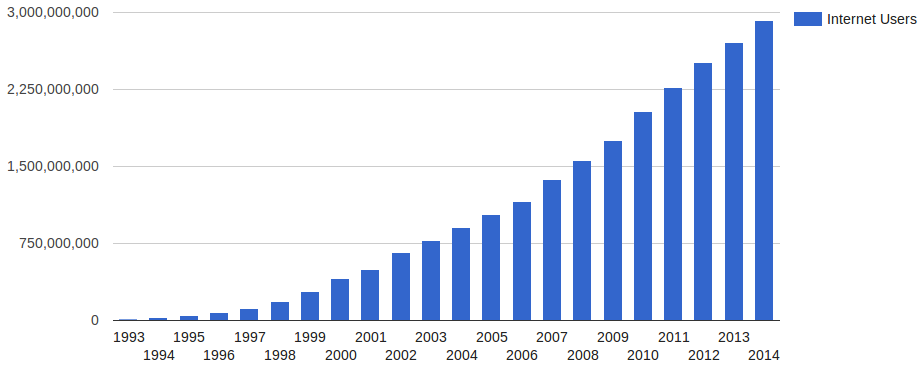
\includegraphics[width=\textwidth]{images/internet_growth}
\caption{The expansion of the Internet}
\label{fig:internet_growth}
\end{figure}

``Network'' is a very generic term. In the IT context, a computer network is set of connected nodes adopting common protocols to exchange data. The most widespread protocol for networking communication is the above-mentioned TCP/IP protocol, that is used in the vast majority of services like the World Wide Web, email, file transfer, remote system access, etc. It is also often used as a communication protocol in private networks and data centers.
The reason for its wide adoption is not that there aren't good alternatives: TCP/IP is not to most performing protocol in every network environment, but it is relatively simple and it introduces fairly low complexity in the overall architecture, still meeting all the most common security and reliability requirements. Back in the 1980s, TCP/IP was the simpler way for applications to use most networks and eventually it was chosen as the protocol for the Internet, thus quickly becoming a de-facto standard \cite{computerworld}.

During its life, the TCP/IP protocol suite has been improved with various updates and additional components to reach the desired levels of network congestion, traffic load balancing, handling of unpredictable behaviors, security, user-experience and so on. Such aspects became more and more challenging with the uncontrollable expansion of the Internet.
Albeit, after all the years that passed since the first implementation, the core components of the TCP/IP protocol design haven't changed at all, mainly for backward compatibility reasons. This inevitably causes some aspects of the old protocol to look very limited in the current networking reality. A well known example is the scarcity of available IPv4 addresses: when TCP/IP was designed in the early stages, a 32-bit number seemed to be a very high number to encompass all the users of the network. Nevertheless, due to the unexpected increase rate in the number of Internet users (and also due to inefficient IP allocation policies), the available IPv4 addresses run out quickly, forcing the introduction of the lengthy 126-bit address format, known as IPv6, formalized in 1998 \cite{rfc2460}. IPv6 is intended to replace IPv4, but the transition towards the new format turned out to be a remarkably complicated procedure overall: IPv6 is not designed to be directly interoperable with IPv4, and even if nowadays the majority of the systems are IPv6-compatible, it took about 20 years to reach the current percentage of overall adoption: 10\% (percentage of IPv6 users accessing Google \cite{google}). This should be a good indicator of the big challenge that is modifying the core design aspects of the TCP/IP architecture, a recurrent topic in this paper.

When the TCP protocol was first developed in the 1970s, it was certainly difficult to predict the rate of growth of the networks around the globe, not only in terms of the number of nodes involved, but also in terms of the quantity and type of the transmitted data, the increasing need of low latency for new streaming applications, the advancement in the hardware adopted to carry the data and the computing power of the interconnected devices. Today we can count billions of interconnected devices, and we have just started the era of the IoT (Internet of Things) which aims at giving communication capabilities to virtually every object commonly used in our daily life.
As a result of this process, the networks are becoming more complex and devices often use multiple interfaces to stay connected. Common appliances like smartphones provide both cellular connectivity and Wi-Fi modules (figure \ref{fig:smartphones}); same technologies can be often found in tablets; laptops have at least Wi-Fi capabilities plus an Ethernet port, and they support third-party receivers for connectivity through cellular networks. The argumentation is much more complex in the backend infrastructures' scenario, which is rapidly evolving due to a new interest in BigData storage and analysis, as well as the flourishing of wide-scale low-latency streaming services (video streaming, VoIP, multiplayer videogames, etc.). Data centers often count tens of thousands of interconnected nodes, often including content-delivery servers that are capable of handling a high number of connections simultaneously.

\begin{figure}[!htb]
\centering
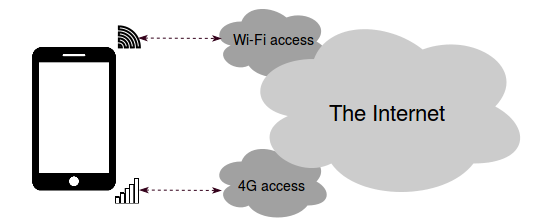
\includegraphics[width=0.75\textwidth]{images/smartphones}
\caption{The typical smartphone connectivity}
\label{fig:smartphones}
\end{figure}

The implications of this new reality include the possibility of establishing multiple paths to transmit data between two applications running on the communicating hosts, since they are now often equipped with multiple network interfaces, each configured with an active IP address. Back in 1970s, TCP was designed to create a virtual connection between exactly two IP addresses and two port values, with almost no flexibility or dynamism in address/port addition and removal within the duration of the connection. In the multipath reality of the infrastructures of today, to old point-to-point single-path connection provided by TCP looks quite limiting. This led to various projects aiming at exploiting the multipath concept, and Multipath TCP is one of them.


Multipath TCP (MPTCP) is an ongoing project managed by the Internet Engineering Task Force (IETF), whose specifications have been published as Experimental Standard in January 2013 \cite{rfc6824}; such protocol extends the current TCP to introduce multipathing capabilities, maintaining backward compatibility at the endpoints and undertaking a major endeavor to avoid disrupting of middleboxes' behavior. MPTPC can communicate with the application layer via standard TCP interface and it automatically splits data at the sender, it sends the data through different subflows (each being basically a regular TCP connection) according to the IP addresses and interfaces available at the hosts and finally reassembles the data at the receiver, in fact enabling multipathing.

\subsection{Benefits of MPTCP}
\label{benefits}
Multipathing provides hosts with the resource pooling concept applied to networking access. Resource pooling allows dynamism and flexibility in requesting and handling resources and it is a positive trend in many services and architectures: Content Delivery Networks (CDNs), Peer-to-Peer (P2P) networks, Cloud Computing, etc. The very concept of packet switching, the core aspect of the modern Internet, is based on a resource pooling technique: circuit utilization is no more performed by allocating isolated channels in the link (static multiplexing) as it was the case with circuit switching, but the traffic is fragmented into small addressed packets that can share the overall link capacity (statistical multiplexing) \cite{DBLP:journals/corr/QadirAYSC15}. MPTCP aims at taking this concept to the next level, by grouping a set of separate links into a pool of links (figure \ref{fig:pooling}).


\begin{figure}[!htb]
\centering
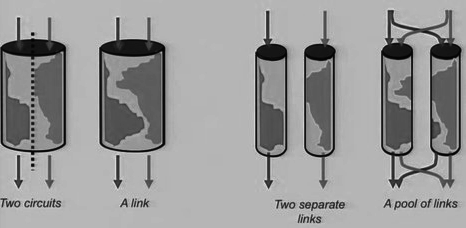
\includegraphics[width=0.75\textwidth]{images/pooling}
\caption{MPTCP pooling principle}
\label{fig:pooling}
\end{figure}


The benefits include better resource utilization, better throughput and smoother reaction to failures, leading to an overall improved user experience, as shown in the following four major use-cases:
\begin{itemize}
  \item Combining MPTCP multipath and multihoming\footnote{Multihoming: the connection to the Internet via multiple providers.}, it is possible to achieve higher throughput by exploiting multiple simultaneous connections to transfer different portions of the same piece of data. For example, a typical smartphone could use its cellular module and its Wi-Fi module simultaneously in downloading a file from a remote server, despite them having two different IP addresses;
  \item It is possible to introduce failure handover for the connection with no special mechanism at network or link layer. If one of the interfaces stops working or the flow of data gets interrupted for any reasons, data transfer can seamlessly continue through other interfaces;
  \item By assigning different priorities to the various flows, it is possible to better handle data transfer through the different interfaces. This could be useful if some connectivity modules drain more battery than others, or if some interfaces are associated to a limited capacity data plan. For example, let's consider the case of a file download on a smartphone via 4G connectivity: it would be advantageous to seamlessly switch the whole data transfer to the Wi-Fi interface if that becomes available in the middle of the download, starting from the point left by the cellular connection and without the need to restart the session;
  \item Providing multipath awareness to current network stacks can improve load balancing and exploitation of the network resources in data centers; this is a valuable aspect, considering that the network performance in data centers is usually critical for maintaining low latency for the overall system. A similar concept applies to load balancing in ISPs' network backbones.
\end{itemize}

\subsection{Multipathing solutions}
\label{mptcp_alternatives}
MPTCP aims at achieving all the benefits mentioned in the previous paragraph by operating at the transport layer of the traditional Internet architecture (the OSI model\footnote{Open System Interconnection model produced at the International Organization for Standardization (ISO): standard model to abstract the communication system of computer networks into different layers of operation without referencing any specific protocol and implementation \cite{osi}.} is shown in figure \ref{fig:OSI}), which is the same layer in which TCP operates.
Before MPTCP, other proposals have been elaborated to achieve multipath benefits by introducing new technologies at the link layer, network layer and transport layer as well. Even at the application layer, developers can create custom frameworks on top of TCP to achieve benefits similar to those that would come by exploiting multipath natively at the lower layers. For example, most modern browsers open many TCP connection simultaneously to download the various elements of a Webpage to improve user experience \cite{Yuchung}. Another example could be Skype and similar VoIP services, which try to automatically reconnect hosts in case of problems with minimum impact on the user experience. Albeit all the solutions at the application layer are just clever workarounds on top of regular TCP and they fall only marginally into our discussion regarding multipath.

\begin{figure}[!htb]
\centering
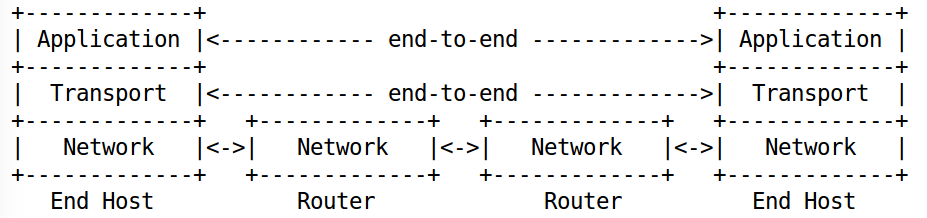
\includegraphics[width=0.75\textwidth]{images/OSI}
\caption{The traditional Internet architecture (OSI model)}
\label{fig:OSI}
\end{figure}

The following list gives a general overview of the most important multipathing solutions other than MPTCP, grouped according to the architectural layer they operate in:
\begin{itemize}
  \item \textit{Link layer}: there are different ways to achieve resource pooling through link aggregation at link layer, but the basic concept is to setup multiple physical links between two logical devices (for example a server and the next-hop switch, or two switches) so that they are bundled in a single \textit{Link Aggregate Group} (LAG) transparently to the higher-level applications. In order for this to work, proper configuration is needed at both the endpoints of the aggregated link, even if a protocol named LACP has been standardized in order to achieve automation in link aggregation configurations \cite{thenetworkway}. It is important to notice that the single data flows are still sent to a single link in the LAG pool in order to maintain sequence-ordering, but overall bandwidth available for all data flows is increased and failover mechanism is really quick and efficient \cite{thenetworkway}. Despite being a common solution in ISPs' inner infrastructure and data centers to improve the bandwidth in specific portions of the network, end users usually cannot directly take advantage of this technology;
  \item \textit{Network layer}: there exist multiple solutions to better exploit multipathing at this layer, most notably \textit{Mobile IP} \cite{rfc5944} and \textit{Shim6} \cite{rfc5533}. Without going into the details, they both provide hot-handover capabilities with no interruption of the higher-level services, with some limitations: Mobile IP requires extensive support by the underlying infrastructure and Shim6 is an IPv6 only solution. More importantly, there is a fundamental problem in confining resource pooling at the network layer: TCP operates at the transport layer but it is closely related to the network layer because it statefully inspects various properties of the underlying network paths to provide performance optimizations (this is why referring to TCP often implies taking into consideration the whole TCP/IP protocol stack): this means that in most cases transparent modifications at the network layer would cause TCP malfunctioning;
  \item \textit{Transport layer}: the most notable experiment in multipath exploitation prior to MPTCP is the Stream Control Transmission Protocol (SCTP) \cite{rfc4960}. Such protocol is, in many ways, similar to MPTCP: the first version of SCTP provided failover capabilities by exploiting different interfaces, and successive versions introduced multi-streaming capabilities to increase throughput. The major problem with SCTP is that it was thought to be an independent, enhanced version of TCP, and the two protocols are indeed incompatible with each other. This means that a wide adoption of SCTP would require to upgrade the networks to be SCTP aware. Moreover, all the applications would need to be upgraded to explicitly switch to the new protocol for communication. The vast global networking scenario of today, mainly based on TCP, makes these requirements virtually impossible to meet, and SCTP remains a technology of very limited adoption \cite{ipspace}.
\end{itemize}

All these previous solutions didn't get widespread adoption. Link layers and network layers solutions require extensive modifications in the underlying network configurations in order to achieve the desired results; introducing a totally new multipath-aware protocol at the transport layer requires to change all the applications in order for them to communicate over the new protocol, thus allowing this solution in very limited scenarios; workarounds at the application layer, despite being quite effective, are far from the purpose of MPTCP.

MPTCP primary goal is to automatically introduce multipath to the infrastructures and devices currently adopting TCP, with the minimum possible effort from users, developers and network maintainers. Engineers decided that the best way to achieve all these requirements was to still use TCP as fundamental block for communication, extending it to support multipath: the entire protocol design works by adding MPTCP custom options into regular TCP segments and each subflow in MPTCP is indeed seen by the lower infrastructure as a regular TCP connection.
MPTCP got a lot of attention in the Internet community in the last few years, and many consider MPTCP as a valuable step forward for the whole global network currently relying on TCP.
The final goal of MPTCP is to replace the majority of the current TCP implementations, which is a very delicate process in which all the current TCP standards in terms of robustness, performance and security have to be maintained, if not improved. This paper is an evaluation of the security aspects of MPTCP, with an analysis of current threats and vulnerabilities affecting the protocol.

\section{Problem statement}
MPTCP is a big effort from the IETF to unlock multipath networking capabilities worldwide, with many subtle implications for current infrastructures. Hence the importance of evaluating the current security status of MPTCP, by inspecting its implications on external middleboxes and security equipment and also by analyzing internal design flaws that might allow attacks to the MPTCP sessions.
The reference implementation for the new protocol is available for the Linux Kernel and currently maintained in an off-tree open-source repository.
The main focus of this paper is related to the main vulnerability currently known for the protocol, concerning the ADD\_ADDR component: during the thesis work such vulnerability is studied and the solution for it is implemented and evaluated. In the process, patches for the Linux Kernel implementation of the protocol have been developed to fix the vulnerability and mark the first step towards the Linux implementation of the new version of MPTCP. The afore-mentioned vulnerability, present in the version 0 of MPTCP, can potentially allow an attacker to perform an off-path hijacking of the connection by exploiting the ADD\_ADDR functionality of advertising the creation of a new subflow: in very simplified terms, the attacker would be able to advertise its own IP address to execute the hijacking.

A comprehensive list of all the objectives for the thesis work is the following:
\begin{itemize}
    \item Studying the security implications of adopting MPTCP on current infrastructures;
    \item Listing the known vulnerabilities affecting the current version of the protocol;
    \item Studying and exploiting the ADD\_ADDR vulnerability of the protocol;
    \item Evaluating the possible solutions for the ADD\_ADDR vulnerability;
    \item Assessing the best solution for the ADD\_ADDR vulnerability and developing it for the Linux Kernel implementation of MPTCP;
    \item Developing effective and powerful simulation scenarios in order to test MPTCP (and possibly other networking protocols);
    \item Contributing to the upstreaming of MPTCP into the Linux Kernel by developing patches and contributing to official RFC documentation.
\end{itemize}

\section{Methodology}
The thesis work has been carried out at the Intel Corporation offices in Lund (Sweden). The process took six months in total, with a main focus on testing and developing. The entire work has been closely followed by major stakeholders in the MPTCP community, located in Sweden, Romania and the United States. Such cooperation involved patch reviewing and weekly meetings.

The engineering approach adopted for the thesis work involved a first major step regarding observations on the protocol's behaviour when subjected to external custom-made input. This step can be considered per se a smaller and modular sub-project, in which it is possible to define yet other sub-steps:

\begin{itemize}
    \item Setting up and running standard MPTCP connections on a portable virtual environment that is fast to manipulate and that provides all the means for proper monitoring and testing of the connections. Such environment had to provide tracing and debugging capabilities for the running Kernel images as well;
    \item Evaluating the best external tools to monitor and observe and capture all the low-level details of the packets exchanged during the MPTCP sessions;
    \item Evaluating the best external tools to easily operate on the ongoing MPTCP sessions, by manipulating and injecting forged packets. Other ways to operate over the connections have been taken into consideration as well, like the firewall setup necessary to block specific kind of packets.
\end{itemize}

These preliminary steps allowed to obtain a fundamental test-bed configuration later adopted extensively during the whole development phase. 
The development phase consisted on a different methodology approach involving multiple iterations. Each iteration consisted on:

\begin{itemize}
    \item Examine the specifications for the required features under development; if present, closely investigate the review and feedbacks from external sources on the ongoing iteration as well;
    \item Apply a relatively small amount of changes to the current implementation according to the previous step;
    \item Extensively testing all the regular and edge cases potentially affected by the modifications elaborated in the previous step (by using the tools from the previously described preliminary steps);
    \item Restart the loop from the first step in case of malfunctioning due to bug in the code; otherwise, changes were pushed into experimental repository for external evaluations, reviews and feedbacks.
\end{itemize}

Despite the iterative approach, the development phase have been arranged to keep good levels of modularity in the produced code, so that each elaborated feature required a certain number of iterations to be completed but the final result could be considered self-contained and valid for all the subsequent features built on top of it. 
Such modularity translated in practice in different patches for the Linux Kernel implementation of MPTCP and allowed for easy selection of the components valuable for the official implementation, while others were saved in experimental branches for future reference.
Each one of the features have been developed starting from the specifications and comments from external sources, and the collaborative environment allowed to reverse the operational flow and occasionally advance proposals more or less formal on modifications regarding the protocol's functioning.
The entire set of iterations and the final patches' submission were followed by a higher-level evaluation of the entire work, that brought up minor issues on the whole project and subsequent faster fixes until the final product was deployed, i.e. all the patches (merged and experimental) were finalized. 

A last major step in the methodology for the work consisted in writing the final report. During such last step, an experimental evaluation on the overall product has been developed to provide additional insights on the performance and functioning changes introduced with the new patches. It is important to mention that no modifications have been applied to the final patches at this stage, since the correct functioning has been positively certified at the end of the development phase, but the additional tests were developed to gather additional data mainly on performance impact.

\begin{figure}[!htb]
\centering
\includegraphics[width=\textwidth]{images/methodology}
\caption{The adopted engineering methodology}
\label{fig:methodology}
\end{figure}

\subsection{Daily workflow}
The workflow started with an overall study of MPTCP and how it interacts with the most common middleboxes. The next step was a more focused evaluation of the current threats for the protocol, mainly referencing to the RFC document regarding such topic \cite{rfc7430}. Within the document, only one vulnerability is considered a blocking issue in the advancement of MPTCP standardization, known as the ADD\_ADDR vulnerability. The document also proposes a change in the protocol design that fixes the problem. With such background, the actual development stage of the work started. At first, it was necessary to sync with the development status by interacting with the official MPTCP mailing list for developers, at \url{https://listes-2.sipr.ucl.ac.be/sympa}. This allowed to make sure that the ADD\_ADDR solution proposed in official documentation \cite{rfc7430} was indeed the preferred one and that nobody started developing a patch for it already.
Before starting to work on the fix, a first stage of the work involved a deeper analysis of the ADD\_ADDR vulnerability: a connection hijacking has been executed by exploiting such vulnerability in a testing environment. This allowed to better validate the criticality of the problem and it was a useful experiment to get acquainted with MPTCP. Moreover, it was a good way to setup a proper testing environment that was then used during the whole patch-development process that followed.

The entire code developed during the stage, around 400 line additions, was eventually merged into the official MPTCP repository for the Linux Kernel. Some additional contributions have been performed in order to improve RFC documentation about the protocol and to upgrade related networking tools to be compatible with the new version of MPTCP.

\subsection{Document structure}
The structure of this paper mainly follows the workflow explained in the previous section. After the introductory first chapter, the discussion is mainly subdivided into two parts: a first part with an analysis about MPTCP background and working principles (chapters 2 and 3); a second part about the original work on simulating and fixing the ADD\_ADDR vulnerability (chapters 4 and 5):

\begin{itemize}
  \item Chapter 2 starts with a broad explanation of the basic concepts of TCP to introduce how MPTCP has been developed on top of it. All the technical details of the new protocol can be found in this chapter, that also includes an analysis on the MPTCP deployment status in the real world and the problematics associated in upstreaming the protocol (mainly incompatibilities with current middleboxes);
  \item Chapter 3 is again a background analysis on MPTCP, with a narrowed focus on security. The chapter includes a comprehensive threats analysis, with an overview of the current security issues affecting the protocol. An entire section is dedicated to the ADD\_ADDR vulnerability. In such section all the details regarding the vulnerability are presented: how to exploit it to hijack an MPTCP connection and what are the requirements  an attacker needs to execute the attack;
  \item Chapter 4 is the first part that introduces the original work carried out during the thesis work. Taking as reference the theory behind the ADD\_ADDR attack explained in the previous chapter, this section explains the development of the script capable of exploiting the vulnerability in a simulated environment. The script code is explained step-by-step, as well as the entire procedure to setup the virtual machines to execute the attack. This entire chapter aims at validating the criticality of the ADD\_ADDR vulnerability and in doing so it also provide setup guidelines for a powerful simulating environment that can be useful for future MPTCP testing and development;
  \item Chapter 5 contains the core part of the thesis work. It starts with a theoretical evaluation of the accepted fix for the ADD\_ADDR vulnerability and it proceeds with its development for the Linux Kernel implementation of MPTCP. All the issues encountered during the project, as well as the required side-features that needed to be implemented for proper functioning, are reported in this chapter. The two last sections of this chapter sum up the contributions produced during the thesis work and provide final evaluation of the performance of the produced patches;
  \item Chapter 6 is the conclusive part of the paper, where related work and proposals for future work are present.
\end{itemize}

\chapter{Multipath TCP}
\label{chap:multipathtcp}

\section{Transmission Control Protocol (TCP)}
MPTCP is an extension of regular TCP, the ubiquitous protocol for highly reliable host-to-host communication in a packet-switched computer network. A proper introduction of the fundamentals of TCP is due.


TCP is a host-to-host communication protocol operating at a layer in between the application program and the Internet Protocol. TCP abstracts all the details of the network connection to the application and it is used at the sender to divide the application data stream into segments that can be efficiently routed through the network after being encapsulated into an IP packet; at the receiver, the segments are reassembled before being sent to the application layer.
The reasons why TCP became a de-facto standard in modern computer communication has been briefly mentioned in the introductory part of the paper. A more technical analysis shows that TCP maintains good levels of reliability for the connection independently from the lower layers it depends on for the raw transmission of bits. TCP is indeed able to handle possible data loss, data damaging, data duplication, out-of-order delivery of data. In order to do this, the data to be transmitted is split into a sequence of TCP segments, each containing an additional \textit{TCP header} with the information needed to operate the protocol functionalities at the nodes. Such functionalities are [\href{https://tools.ietf.org/html/rfc793}{ref}]:

\begin{itemize}
  \item \textit{Basic data transfer}: sending continuous stream of octets in each direction between its users, identified by the 4-tuple: source IP address, source port, destination IP address, destination port. The IP address allows to route packets to the destination machines, while the port values direct the content of the packet to the right application within a host;
  \item \textit{Reliability}: in-order, reliable data transfer is achieved by adding a sequence number to each transmitted octet and using ACK signals and timeouts to possibly trigger retransmission of lost packets. TCP assures that no transmission errors will affect the delivery of the data if the network is not completely partitioned;
  \item \textit{Flow control}: the receiver can control the amount of data sent by the sender in a certain moment of the connection by returning a "window" value in the TCP header, so that it is possible to avoid buffer congestion;
  \item \textit{Multiplexing}: a single host is allowed to use multiple independent TCP connections simultaneously thanks to the port value available in the protocol. This value, together with the host address assigned at the internet communication layer, forms a socket, that is the actual endpoint of a TCP connection;
  \item \textit{Connections}: TCP initializes and maintains status information regarding each connection and the data stream between a pair of sockets in order to provide all its functionalities. Such status information is initialized during a first handshake procedure, and released only upon connection termination. TCP is indeed known as a virtual-connection protocol;
  \item \textit{Precedence and Security}: these aspects refer to the possibility of prioritize connections and assign security properties to them. Both precedence and security can be configured by users, but default values are provided.
\end{itemize}

As noted above, all these features are made possible by processing the bits at the TCP header. Such structured set of information is mostly static and predefined, so that at each position in the header corresponds a well known portion of the protocol data. The TCP header looks like the one in Figure \ref{fig:tcp_header}.

\begin{figure}[!htb]
\centering
\includegraphics[width=0.75\textwidth]{images/tcp_header}
\caption{The TCP header format}
\label{fig:tcp_header}
\end{figure}

There are 10 mandatory fields in the TCP header.
The \textit{Source Port} and \textit{Destination Port}, together with the source and destination IP addresses provided in the upper IP header (not shown in figure \ref{fig:tcp_header}), are the means for identifying the two endpoints of the TCP connection. \textbf{These static fields clearly shows the single-path fundamental design of the protocol}. 


TCP assures reliability standards independently from the lower layers used to route packets and transmit raw bits, and it is possible that packets arrive at destination unordered, or that some of them are lost on the way; \textit{Sequence Number} and \textit{Acknowledgment Number} are used in TCP for such cases: numbering each octet it is possible to put them in sequence and acknowledge them in a cumulative way, so that by acknowledging sequence number X means that all packets up to but not including X has been received. This system, together with timeouts, allows for retransmission of lost packets. For security reasons, numbering starts with a random 32-bit value that is agreed upon TCP connection three-way handshake. There are flag bits used to determine if a TCP segment is an ACK segment, so that in those cases the \textit{Acknowledgment Number} indeed represents the next \textit{Sequence Number} that the receiver is expecting. Among the other flags in the TCP header there are the following:
the SYN flag is sent only for the first packet of each host and it is used during the initial TCP handshake; the FIN flag is used to indicate that the sender is sending no more data, thus playing a fundamental role in the connection's tear down; the RST flag is used for segments that are forcing a reset for the connection.


The \textit{Window} field, which allows to achieve congestion control by telling to the sender the range of sequence numbers the data receiver is prepared to accept in a particular instance of time. The \textit{Checksum} field guarantees that data has not been modified on its way to the destination, intentionally or unintentionally (thus being part of the reliability aspect of the protocol). A component of the TCP header that is fundamental for MPTCP is the \textit{Options} field, which was firstly introduced as a free space for future additions to the protocol. In this specific case, the TLV solution is adopted to process the data inside the field. "TLV" stands for \textit{type-length-value}, where the type is the ID value uniquely identifying the option, the length is the number of bytes of the option, whereas the value represents the actual option content. This particular design allows to skip unknown options at the receiver by simply checking the length value and moving the pointer accordingly. An important limitation for this field is that its total length cannot be more than 40 bytes [ref].

\section{MPTCP design}
MPTCP \textit{functional goals} are to increase resilience of the connectivity and efficiency of the resource usage by exploiting multiple paths (subflows) for the connection.
Such goals can be found very similar in other multipathing solutions as the ones described in section [add section], but what is really unique about MPTCP protocol design is the set of its \textit{compatibilities goals} [\href{https://tools.ietf.org/html/rfc6182}{ref}]:

\begin{itemize}
  \item \textit{Application compatibility} aims at instantiating a protocol that can be fully operational with no modifications for the applications using it. This means that the networking APIs and the overall service model of regular TCP has to be maintained with MPTCP; the entire MPTCP functioning is handled transparently by the underlying system. Such transparency must be maintained also in terms of throughput, resilience and security for the connection, that cannot be deteriorated with respect to the current TCP standards;
  \item \textit{Network compatibility} is a goal similar to the previous one, since MPTCP is supposed to work out of the box with the current underlying network layer and the ones below it. The main reason still resides in the possibility of achieving a smooth wide-spread deployment of the protocol on the current infrastructure;
  \item \textit{Users compatibility} is a corollary to both network and application compatibility, which states that MPTCP flows must be fair to regular TCP connection in case of shard bottlenecks.
\end{itemize}


All these compatibilities requirements should explain the very fundamental decision of developing the new multipath protocol at the transport layer, and more specifically as an extension of regular TCP. Let's take into consideration the traditional TCP protocol stack and compare it to the new MPTCP stack (figure \ref{fig:stack}).
To achieve the required compatibility goals, changes had to be applied to layers lower than the application layer, so that current programs do not have to be upgraded to make use of multipath; on the other side, the new protocol had to be placed at layers above the network layer, which is the last layer still operating at the network infrastructure before the transport layer, the latter being the first layer operating at the end systems. The idea with MPTCP is to deploy it as a simple upgrade of the end systems' OS, with no modifications applied to the network infrastructure.

\begin{figure}[!htb]
\centering
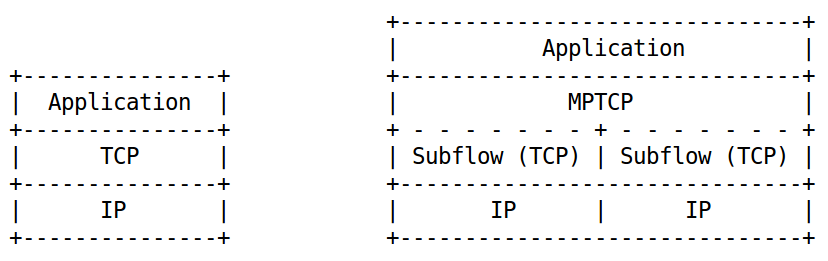
\includegraphics[width=0.75\textwidth]{images/stack}
\caption{The TCP and MPTCP protocol stacks}
\label{fig:stack}
\end{figure}

The choice of working at the transport layer was indeed the only available option. Within that option, the choice of maintaining TCP as the fundamental operating protocol for MPTCP was still straightforward for similar compatibility reasons; for this very purpose engineers decided to add all the required options for MPTCP inside the TCP \textit{Option} field in the TCP header. In this way, MPTCP-aware systems can process the MPTCP options for multipathing, but if a system that is not MPTCP-aware receives a MPTCP connection-request, it would simply discard the MPTCP options and treat such message as a plain TCP connection-request. 
MPTCP design maintains the behavior of the subflows to be compliant with regular TCP, while reassembling of data incoming from different paths is a process executed by the receiving host only. MPTCP subflows are indeed seen by middleboxes as regular and independent TCP connections carrying additional options. If security policies at the middleboxes is not too restrictive against unknown options, MPTCP-unaware nodes would still work with the new protocol.
For what regards applications, they don't need to be changed either since MPTCP would be inserted into the network stack at the operating system level: it would automatically split the data buffered from the application layer and send it through different subflows, according to the number of available endpoints at the connected hosts. Communication with the application layer can be performed through the old TCP APIs, even if MPTCP specific options can be used by upgraded user programs to take advantage of more advanced options in MPTCP.

A functional decomposition of MPTCP brings up four core functions the protocol offers:
\begin{itemize}
  \item \textit{Path management}: MPTCP has to provide a mechanism to detect and use multiple paths between two hosts;
  \item \textit{Packet scheduling}: MPTCP fragments the byte stream received from the application in order to transmit it through different subflows, adding the required sequenced mapping used to reconstruct the same byte stream at receiver. This function of MPTCP adopts the information from the path management component to exploit the different paths;
  \item \textit{Subflow interface}: as mentioned multiple times, MPTCP uses TCP to send data in a single subflow;
  \item \textit{Congestion control}: a congestion control mechanism at the MPTCP connection layer is needed to make sure that MPTCP wouldn't starve a singlepath TCP flow in a shared bottleneck. The congestion control component is the way MPTCP schedule segments at the various subflows, also taking into account the scheduling rate.
\end{itemize}

The previous functions of MPTCP are implemented internally at each host and they use a relatively compact set of TCP options to operate between two hosts. Technically, there is only a single generic MPTCP option, to which has been assigned the value 30 as the TCP "Option-Kind" identifier; at a lower level it is possible to identify a set of eight MPTCP option subtypes, each identified by a 4-bit value (this classification, reported in figure \ref{fig:MPTCP_options}, references to \rfc{6824}). 

\begin{figure}[!htb]
\centering
\includegraphics[width=0.75\textwidth]{images/MPTCP_options}
\caption{The set of MPTCP options [RFC-6824]}
\label{fig:MPTCP_options}
\end{figure}

\subsection{Control plane}
The control plane for MPTCP takes into consideration all the options used in MPTCP to handle connection initiation, addition and removal of subflows, priority assignment to specific subflows, error handling via 'fallback' mechanism. These options are reported in the following subsections, adopting as reference documentation the \rfc{6824}.

\subsubsection{MP\_CAPABLE}
The connection initiation of an MPTCP connection is very similar to the standard TCP initial three-way handshake, involving a SYN, SYN/ACK and ACK exchange on a single path between host A and host B. In a regular TCP connection establishment these three packets are used to guarantee that both hosts have received an acknowledgment of the connection and also to exchange the two random initial sequence numbers that will be used to acknowledge data delivery for the two directions of the connection. Despite working as regular TCP packets, if MPTCP is enabled the SYN packet from host A will have a MP\_CAPABLE option in the \textit{Options} field of the TCP header; if the receiver host B is not MPTCP-compatible it will simply discard the MP\_CAPABLE option and proceeds instantiating a regular TCP connection.
In case both hosts are MPTCP-compatible, the MP\_CAPABLE option is inserted in the three packets of the initial handshake for two purposes: advertise that both hosts are indeed MPTCP-compatible and allow them to exchange two 64-bit keys (Key-A and Key-B), according to the scheme in figure \ref{fig:mpcapable}.

\begin{figure}[!htb]
\centering
\includegraphics[width=0.75\textwidth]{images/mpcapable}
\caption{MPTCP connection initiation}
\label{fig:mpcapable}
\end{figure}

These keys are sent in clear inside the MP\_CAPABLE option only during the initial handshake and their purpose is to identify a specific MPTCP connection within a host (useful when associating a new subflow to an existing MPTCP connection, for example) and to provide shared security material that is used in MPTCP for authorization mechanisms (more on this later in this section). The \textit{Option} field in the TCP header can only be 40 bytes long, and it is not reserved to MPTCP only. For this reason it is of primary importance to keep the amount of MPTCP related metadata as low as possible. In fact, the original 64 bit keys are exchanged only during initial handshake; subsequently, shorter 32 bit tokens (Token-A and Token-B) derived from such keys will be used to address a specific MPTCP connection, even if this procedure requires additional checks in case of collisions with other tokens already assigned to other MPTCP connections in the same machine. Therefore, an implementation will require a mapping from each token to the corresponding connection, and in turn to the keys for the connection.


Regarding the hashing algorithm used to produce the tokens, this can be negotiated by using a portion of the flag bits inside the MP\_CAPABLE option. In this paper, the SHA1 (and HMAC-SHA1 in case a key element is needed) is considered [ref to SHA1]. Note that the SHA1 algorithm produces a 160-bit / 20-octet resulting value, that is then truncated to its leftmost 32 or 64 bits according to the different cases in the MPTCP operations.

\begin{figure}[!htb]
\centering
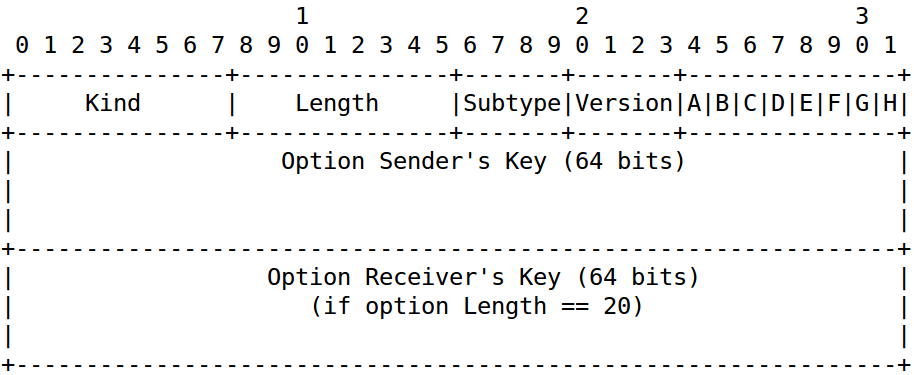
\includegraphics[width=0.75\textwidth]{images/opt_capable}
\caption{MP\_CAPABLE option}
\label{fig:opt_capable}
\end{figure}

\subsubsection{MP\_JOIN}
Suppose that after the first subflow is operational host A initiates a new subflow between one of its addresses and one of host B's addresses (figure \ref{fig:mptcpauth}). Host A sends a TCP SYN packet to host B containing the MP\_JOIN option, which includes Token-B (the token derived B's key) and a nonce value used to prevent replay attacks. An additional field in the MP\_JOIN option is called Address ID, an identifier for the original addresses in use within a single MPTCP connection; this additional value allows to refer to a specific subflow without the need to use the addresses as identifiers, which is very useful when middleboxes like NATs alter the IP header during the transit of the packets.

At the lower layers of the network, the SYN packet sent in this way looks like a legitimate request from host A to initiate a new TCP connection with host B, being the SYN packet the first of the regular TCP initial handshake. Host B treats such packet as a new MPTCP subflow request, and it uses the Token-B in the packet to associate the request to the specific ongoing MPTCP connection with host A.

The handshake flow for MP\_JOIN includes HMAC values for authentication purposes, and it is structured as follow:
\begin{itemize}
  \item Token-B is added in the SYN packet from host A to host B in order to address a specific MPTCP connection; a random nonce (R-A) is also sent along;
  \begin{figure}[!htb]
\centering
\includegraphics[width=0.75\textwidth]{images/opt_join1}
\caption{MP\_JOIN option - SYN}
\label{fig:opt_join1}
\end{figure}
  \item Host B processes the request and sends back a truncated HMAC value calculated by using as \textit{key} the concatenation of Key-B followed by Key-A, and as the \textit{message} the concatenation of a new nonce computed at host B (R-B) and the one received from host A (R-A). R-B is also added to the packet, since it is needed by host A in the next step;
\begin{figure}[!htb]
\centering
\includegraphics[width=0.75\textwidth]{images/opt_join2}
\caption{MP\_JOIN option - SYN/ACK}
\label{fig:opt_join2}
\end{figure}
  \item The last ACK form host A to host B only has to contain the HMAC calculated using as key the concatenation of Key-A and Key-B, and as message the concatenation R-A and R-B. This time, the HMAC value is sent in its full length of 160-bit.
\begin{figure}[!htb]
\centering
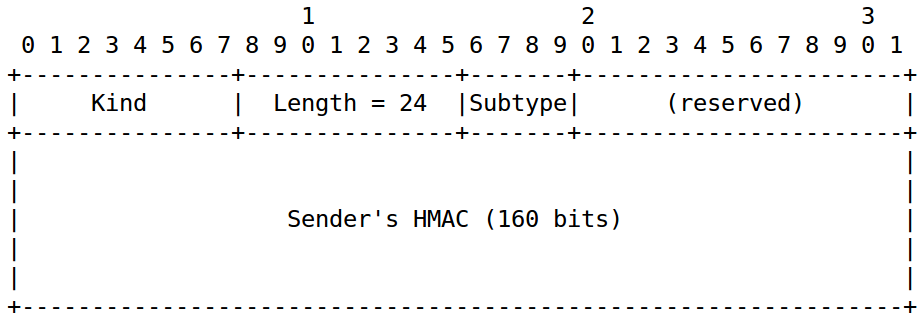
\includegraphics[width=0.75\textwidth]{images/opt_join3}
\caption{MP\_JOIN option - ACK}
\label{fig:opt_join3}
\end{figure}
  \item Note that the HMAC in the ACK packet from host A to host B has to be acknowledged for the subflow to be finally established. This because the third ACK is the only packet where the HMAC from host A is sent, and it has to be acknowledged or retransmitted is the fourth ACK from host B is not received.
\end{itemize}

These HMAC values are used to authenticate the participants in the subflow establishment, since both have to know the keys for the MPTCP connection. If the creation of the new subflow is not possible because A sends an unknown Token-B to host B or the HMAC material exchanged is not recognized by either hosts or the SYN/ACK received at host A misses the MP\_JOIN option, then the operation is stopped sending a TCP RST.


If everything works properly, the entire procedure of instantiating a MPTCP connection and add a subflow is represented with the example in figure \ref{fig:mptpcauth}. 

\begin{figure}[!htb]
\centering
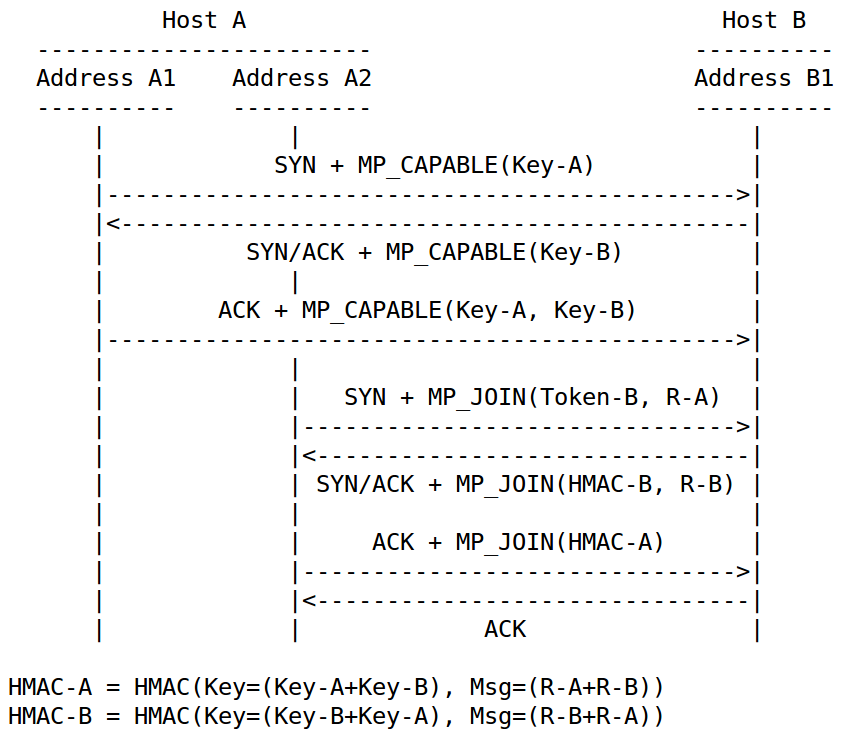
\includegraphics[width=0.75\textwidth]{images/mptcpauth}
\caption{MPTCP authentication example}
\label{fig:mptcpauth}
\end{figure}


\subsubsection{ADD\_ADDR}
Even if a host can directly instantiate a new subflow using the MP\_JOIN option as previously described, another possibility is for the host to advertise an available address to the other machine, thus allowing the latter to instantiate the subflow.
This functionalities can be useful, for example, in a typical client-server Web configuration in which only the client is allowed to open new connections with the server: if a new interface becomes available at the server, it can dynamically advertise it to the client which in turns can send the SYN+MP\_JOIN packet for subflow initiation.


This functionality is provided in MPTCP by the ADD\_ADDR option, that indeed contains the additional address (and, optionally, port) to be advertised. The option also includes the previously mentioned Address ID value, that has to uniquely address the address to the sender (within the same MPTCP connection).


The ADD\_ADDR option is treated as a soft component of the overall architecture, with no need to be sent reliably and/or be acknowledged by the receiver. The option can be added to any packet in the MPTCP connection if there is enough space in the \textit{Option} field of the TCP header, with no guarantee that such option will be received or that the receiver will indeed use the advertised information to start a new subflow. This low priority assigned to ADD\_ADDR is reasonable since the malfunctioning of this option would not break the overall data transmission, but it might only cause a missed opportunity for better multipath exploitation. For similar reasons, there is no need to ensure a proper ordering for ADD\_ADDR and REMOVE\_ADDR at the receiver (REMOVE\_ADDR, explained in the following subsection, is similar to ADD\_ADDR but it indicates which subflow to shut down instead). Albeit the typical TCP validity test will be performed before inspecting the ADD\_ADDR option.

The content of the ADD\_ADDR option is shown in figure \ref{fig:addaddropt}. The IPVer indicates if the advertised address is of kind IPv4 or IPv6, while the other fields contain the Address ID, Address and optional port as previously stated.

\begin{figure}[!htb]
\centering
\includegraphics[width=0.75\textwidth]{images/addaddropt}
\caption{ADD\_ADDR option}
\label{fig:addaddropt}
\end{figure}

\subsubsection{REMOVE\_ADDR}
If an address becomes unavailable during a MPTCP connection, the affected host should announce this so that any subflow currently using that address can be terminated. For security purposes, when a REMOVE\_ADDR is received, a test is performed to make sure that the address is not available anymore, by sending a TCP keepalive on the path.
The Address ID is used to identify the path to be shut down, so that no explicit address is needed (and no address is indeed present in the REMOVE\_ADDR option), and the option would work through NATs as well. 
A subflow that is working properly must not use this option to close the connection, but a FIN exchange similar to regular TCP is performed instead.

\begin{figure}[!htb]
\centering
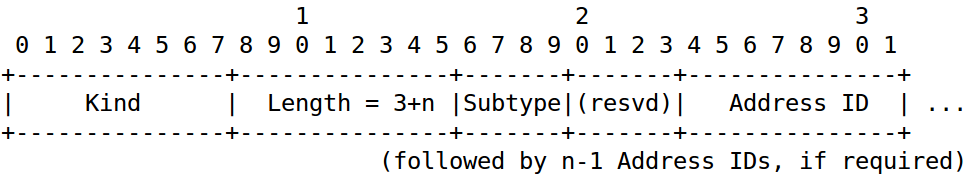
\includegraphics[width=0.75\textwidth]{images/opt_remove}
\caption{REMOVE\_ADDR option}
\label{fig:opt_remove}
\end{figure}



\subsubsection{MP\_FASTCLOSE}
This option can be thought as the MPTCP-level counterpart of the RST signal for the TCP connections: it permits the abrupt closure of the whole MPTCP connection. The RST signals couldn't trigger such behavior, since they are confined to work against a single TCP flow (i.e. MPTCP subflow).

This option can be sent by host A to trigger MPTCP closure at host B. In this case, MP\_FASTCLOSE must contain the value of Key-B. When host B receives the option through one of the subflows, it will send a TCP RST answer via the same subflow and then tears down all the subflow. Host A is waiting for the TCP RST answer from host B before tearing down all the subflows. This generic behavior might change slightly if both hosts send an MP\_FASTCLOSE at the same time, or if the awaited TCP RST signal is not received within a certain timeout (these would trigger a limited number of retransmissions for this option).

\begin{figure}[!htb]
\centering
\includegraphics[width=0.75\textwidth]{images/opt_fastclose}
\caption{MP\_FASTCLOSE option}
\label{fig:opt_fastclose}
\end{figure}

\subsubsection{MP\_FAIL}
There are various cases in which things might go wrong for a MPTCP connection, and the right procedure to handle such cases is to 'fall back', meaning either falling back to regular TCP or removing the subflow generating the issue. The first solution we saw already for the MP\_CAPABLE case, where TCP fall back is guaranteed in case a host is not MPTCP compatible. Similarly, subflow addition will be blocked if anything goes wrong in the MP\_JOIN packets' exchange procedure. However, there are other cases in which problems occur after this initiation phases, on regular packets.


As explained in section [ref to section "Data plane"], data acknowledgment with MPTCP requires a DSS option present in the ACK packets. If that option is missing, the path is not considered MPTCP capable. The consequences are different according to the subflow: if the affected path is the first instantiated with the MP\_CAPABLE option then it must fall back to regular TCP; any other subflow showing such problem would be closed with a RST. 
Fallback can be required at any point during the connection if a middlebox modifies the data stream. This case would be detected thanks to the checksum properties of MPTCP data transfer. If checksum fails, all data from the failing segment onwards cannot be trusted anymore. When this happens to a subflow, that has to be immediately closed with a RST and a MP\_FAIL option that indicates the data sequence number that failed the checksum. Such option indeed contains a single main field storing the full 64-bit sequence number. The receiver can then avoid to acknowledge untrusted data, that will be sent again through a different subflow following the retransmission features of the data plane part of the MPTCP protocol. After the fallback to regular TCP, it is mandatory not to revert back to MPTCP later on in the connection.


\begin{figure}[!htb]
\centering
\includegraphics[width=0.75\textwidth]{images/opt_fail}
\caption{MP\_FAIL option}
\label{fig:opt_fail}
\end{figure}

\subsubsection{MP\_PRIO}
It is possible to indicate if a path has to be used regularly or just as backup in case there no other available regular paths. This preference can be advertised at subflow creation via a flag in the MP\_JOIN option, but it is also possible to signal a priority change during the whole time of the MPTCP connection. In fact, it is enough to send the MP\_PRIO option to the targeted subflow to switch priority, to signal the other host about the change; it is also possible to add an Address ID to the option to target all the subflows using the addresses associated to such Address ID. This option is only sent from the receiver to the sender, even if the sender can discard such priority preference for any reasons. 


\begin{figure}[!htb]
\centering
\includegraphics[width=0.75\textwidth]{images/opt_prio}
\caption{MP\_PRIO option}
\label{fig:opt_prio}
\end{figure}

\subsection{Data plane}
This part concerns all the MPTCP options used to manage the data flow in a MPTCP connection, including how the byte stream is subdivided into different subflow and how the original order of the packets is provided at the receiver.

\subsubsection{DSS option}
In order for the receiver to reassemble the correct data stream in MPTCP, a specific option called DSS is used. This option contains the data mapping and Data ACK: data mapping is used to map the sequence space at each subflow (which is independently handled by the TCP protocol) to the overall sequence space at connection level; Data ACK is the procedure to acknowledge data receipt at connection level in MPTCP.
The DSS option can also signal the equivalent of a TCP FIN for the overall MPTCP connection, meaning that the current mapping covers the final data from the sender (figure \ref{fig:mptcp_fin}). 

\begin{figure}[!htb]
\centering
\includegraphics[width=0.75\textwidth]{images/mptcp_fin}
\caption{Closing a MPTCP connection}
\label{fig:mptcp_fin}
\end{figure}

This option might also include the checksum field to perform integrity checks on the payload (if this was enabled when instantiating the connection via the MP\_CAPABLE option).
DSS is indeed a versatile packet, whose per-packet behavior is mainly defined by the appropriate flags (figure \ref{fig:opt_dss}). 

Regarding the data sequence mapping in MPTCP, the general idea is to maintain TCP-compliant and independent sequence numbers for the single subflows, while using a mapping functionality at the MPTCP-level, provided by the DSS option, to properly rearrange the data at the receiver at guarantee in-order and reliable overall transmission as in the case of legacy TCP. The alternative approach would have been to have a single MPTCP-level sequence number used for the entire set of subflows, meaning that a single subflow inspected by middleboxes at the network infrastructure would look like a TCP connection with holes in the payload delivery; this could trigger unwanted behaviors that would be against the compatibility goals towards the current networks.


The DSS option achieves data sequence mapping with the combination of three fields: for a certain number of bytes (indicated in the \textit{Data-Level Length field}, and starting from the reported subflow sequence number (\textit{Subflow Sequence Number} field), the TCP-level sequence maps to the MPTCP-level sequence with starting value indicated in the \textit{Data sequence number} field.
The \textit{Data ACK} field works as regular TCP ACK value, but it refers to the MPTCP-level acknowledgment of the received data. Note that subflow-level acknowledgement is still provided by regular TCP, but a second acknowledgement mechanism at connection-level is desired, since there might cases in which data that has been acknowledges at the subflow-level can be discarded in the buffers before reaching the application. By following the core principles of MPTCP, retransmission of packets can occur at different paths.

\begin{figure}[!htb]
\centering
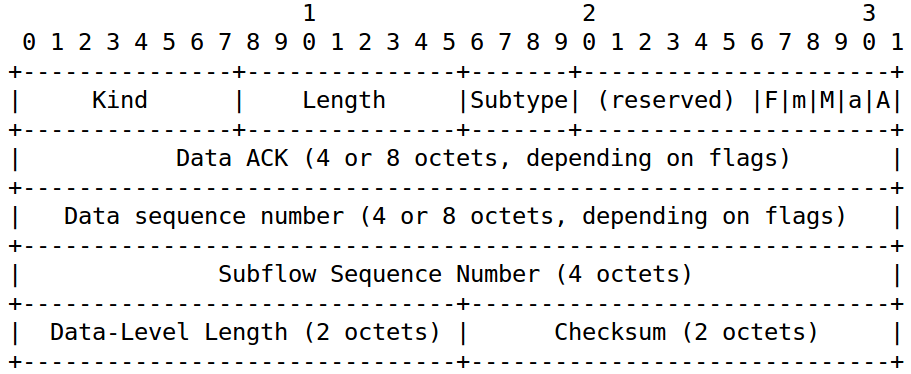
\includegraphics[width=0.75\textwidth]{images/opt_dss}
\caption{DSS option}
\label{fig:opt_dss}
\end{figure}

\section{MPTCP deployment}
A seamless transition to MPTCP on current infrastructures is a major requirement for MTPCP deployment.
Despite the big effort in designing a protocol compliant with strict compatibility requirements, assuring correct functioning in all the current network scenarios is not a viable possibility for MPTCP. The main problematics are related to unwanted behavior of middleboxes processing unknown MPTCP packets, but that is not the only aspect currently limiting the deployment status of the new protocol. MPTCP has to guarantee the same levels of reliability, performance and security of regular TCP (including the cases in which the fallback mechanism is adopted to switch to plain TCP). 
For these reasons, MPTCP includes various mechanisms to cope with the most common middleboxes of today's Internet, including the possibility to detect when external boxes operate on the traffic in a way that cannot be handled by MPTCP thus triggering fallback to regular TCP.


\subsection{Middleboxes compatibility}
The Internet at its core was designed to provide end-to-end connectivity across an infrastructure of interconnected routers. Nevertheless, the growing rate of adoption and increasing complexity of the Internet brought up a wide set of new requirements inherent the intermediate stages of the communication rather then the end-hosts. Such requirements include the need to instantiate protection techniques against potential attacks, more flexibility in content delivery, caching for more efficient communication; they can even be more specific, like the need to rapidly overcome the previously mentioned IPv4 addresses depletion. Middleboxes are pieces of equipment that operate on the network traffic to meet these requirements. The most common middleboxes are NATs, proxies and firewalls, but nowadays there is a huge variety of deployed middleboxes that inevitably break the end-to-end principle of the Internet. Despite their usage is often required, they are more or less intrusive at different layers of operation (according to where they operate within the OSI architectural model), thus causing malfunctioning of many protocols, and MPTCP is no exception. Middleboxes can indeed inspect packets, re-route them, drop them, split them into multiple fragments, and even modify single fields in packets' headers (like rewriting sequence number or removing TCP options) as well as change their payload.


The various operations and purposes of middleboxes are many and often mixed together to achieve more complex policies, and it is also very common that different kind of operations are performed inside the same physical machine. Despite this, it is possible to define a set of most common distinct middleboxes' operations [\href{https://queue.acm.org/detail.cfm?id=2591369}{href}]. 

\subsubsection{Firewalls}
A simple example can be the case of a standard firewall that is not MPTCP-aware and its default policy is set to "Deny". In this case, all the traffic is blocked unless the set of custom rules configured in the firewall explicitly allows a specific typology of packets. In this case, specific for MPTCP must be added to support the new protocol, and this might cause a considerable effort for network maintainers. For example, it is often not straightforward to operate on legacy firewall configurations for big companies with many access points.
A more subtle problem with firewalls might be derived by the fact that they can sometimes manipulate the sequence numbers of a TCP connection, thus moving the sequence number space with respect to the initial value in use by the end-hosts. This feature has been introduced in the past to improve security with older TCP/IP stacks, but the concept can disrupt MPTCP mapping between subflow sequence number and MPTCP-level sequence number. To avoid such problems, MPTCP is designed so that the mapping in the DSS option is using relative values compared to the initial sequence number and functioning is not jeopardized but changes of the absolute values performed by the firewalls.
Yet another case concerns firewalls that remove unknown TCP options for security purposes. If such operation is symmetric, TCP segments would lose the MP\_CAPABLE option and fallback seamlessly to regular TCP. However, there are middleboxes that operates asymmetrically thus removing unknown TCP options only fro non-SYN segments. To cope with this, MPTCP requires that for the first window of data, each segment must include an MPTCP option, otherwise fallback is assured [\href{http://conferences.sigcomm.org/co-next/2013/workshops/HotMiddlebox/program/p37.pdf}{href}].

\subsubsection{NATs}
Another ubiquitous piece of equipment is the "Network Address Translation" (NAT). As the name suggests, NATs modify the IP addresses within the packets on their way towards the destination. The main purpose is to group addresses of an internal private network and map them to a single public address before forward the traffic to the Internet. NATs are also able to redirect the response from the Internet to the right host in the internal network.
This procedure became very common with the depletion of IPv4 addresses, since in many cases the address space assigned to a outer portion of the Internet is not large enough to cover the number of hosts willing to acquire connectivity. 
NATs turned out to be a very effective way to temporarily solve the problem of IPv4 addresses, but their mode of operation is intrusive at the network and transport layer, since the IP addresses are not fixed anymore.
For example, even if NATs use internal tables to keep track of the mappings and are able to redirect replies from the external network to the right internal host, it is no more possible for the external hosts to instantiate a new connection with a specific host residing behind a NAT. This is true also in MPTCP, such that a server often cannot open a new subflow with a client if the latter is behind a NAT, even if a valid MPTCP session between client and server is already active. This is one of the main use cases in which an ADD\_ADDR message can be sent on live subflows in order to trigger a new subflow connection request from the other side.
Moreover, to cope with NATs that might be operational on the paths and might change the source address of the packets, MPTCP refers to addresses by using an Address ID, as previously mentioned in the section [add ref to control plane]. 

\subsubsection{Segment splitting and coalescing}
There are middleboxes that split segments on the Internet as required by the MTU (maximum transmission unit). This means that the payload of a single TCP packet can be scattered across multiple smaller TCP packets and regrouped back together by using the appropriate TCP fields in the header. This operation usually copies TCP options unchanged into each of the smaller packets that are generated. By simply adopting data-sequence numbers in a MPTCP option, the receiver might receive different packets with the same data-sequence numbers and it would be unable to reconstruct the original data. MPTCP takes care of segment splitting and coalescing by mapping the subflow-level TCP sequence number with the MPTCP-level sequence, by providing both the beginning (with respect to the subflow sequence number) and the length of the of the data-sequence mapping [section about DSS].
MPTCP would work also in the more uncommon cases in which segment splitters copy the original TCP option in only one of the generated smaller segments. If the first data-segment does not contain an MPTCP option, fallback to regular TCP is performed (as explained in 'Firewalls' section), otherwise MPTCP would work seamlessly even under these circumstances [\href{http://conferences.sigcomm.org/co-next/2013/workshops/HotMiddlebox/program/p37.pdf}{href}].

\subsubsection{Application-level gateways}
There are middleboxes that operate at higher layer in OSI model, modifying the payload of the packets: adding and removing bytes can change the boundaries of the data-sequence mapping and MPTCP information about it would become inconsistent. The only way to cope with this case is to fallback to regular TCP. In order to that, MPTCP has to detect when the payload has been changed by middleboxes and that is the main reason for which the checksum field has been added inside the DSS option [ref to DSS section]. The checksum calculation is optional in MPTCP and can be negotiated during connection establishment with a flag in the MP\_CAPABLE option. Nevertheless, it is recommended for operations on the open Internet.


\subsection{Deployment status}
MPTCP proves to be a major TCP extension, and in this regards its design required a lot of efforts and several interconnected research projects. The European Commission funded the work at the Université catholique de Louvain with the FP7 Trilogy project in 2007 [\href{http://www.trilogy-project.org/}{href}], followed by CHANGE [\href{http://www.change-project.eu/}{href}] and Trilogy 2 [\href{http://trilogy2.it.uc3m.es/}{href}]. Fundings have been instantiated by Google and Nokia, too [\href{https://multipath-tcp.org/pmwiki.php}{href}]. 

Also by analyzing the main steps in MPTCP evolution we can detect the big interested in the protocol: six month after the Experimental standard for MPTCP has been published in January 2013 by the IETF, it was possible to count three major independent MPTCP implementations other than the Linux kernel implementation [\href{https://datatracker.ietf.org/doc/draft-eardley-mptcp-implementations-survey/?include_text=1}{href}], including a FreeBSD implementation from Swinburne University of Technology [\href{http://lists.freebsd.org/pipermail/freebsd-net/2013-March/034882.html}{href}] and a NetScalar Firmware implementation from Citrix Systems [\href{https://www.citrix.com/blogs/2013/05/28/maximize-mobile-user-experience-with-netscaler-multipath-tcp/}{href}].
Moreover, recent versions of MPTCP kernel (from 0.89.5) are now compatible with Android (with some limitations), and many porting projects have been developed to test older versions of MPTCP on various Android devices [\href{https://multipath-tcp.org/pmwiki.php?n=Users.Android}{href}].
As of June 2015, a Solaris implementation is reportedly under development by Oracle [\href{https://mailarchive.ietf.org/arch/msg/multipathtcp/ugMIu566McQMn8YCju-CTjW9beY}{href}].
All these implementations follows the standard RFC documentation for MPTCP, and they have shown good interoperability capabilities while operating with the standard MPTCP-compatible Linux kernel, especially for what regards the core MPTCP signaling messages (secondary MPTCP features like ADD\_ADDR address advertisement are not always implemented [\href{https://datatracker.ietf.org/doc/draft-eardley-mptcp-implementations-survey/?include_text=1}{href}]).


The very first large scale commercial deployment of MPTCP dates back to 2013, when Apple introduced the new protocol in iOS7 to work with the intelligent personal assistant Siri. Apple's mobile operating system implements MPTCP as in \rfc{6824} (excluding some features) in order to use cellular data subflow in case the Wi-Fi connectivity becomes unavailable during a Siri request processing [\href{https://support.apple.com/en-us/HT201373}{href}]. This is indeed the first example of wide adoption of MPTCP over the Internet even if limited to a specific Apple service connecting to proprietary servers. Nevertheless, the news was helpful in spreading the awareness about the protocol also to a more consumer-oriented audience. Apple also added MPTCP capabilities to Mac OS X 10.10 in October 16, 2014 [\href{http://labs.neohapsis.com/2014/10/20/mptcp-roams-free-by-default-os-x-yosemite/}{href}], proving to be very active in developing and testing MPTCP.


In studying the protocol's deployment process, it is very important to analyze the relation between costs and benefits that MPTCP would bring to each and every group of MPTCP stakeholders.
The success of MPTCP depends on its deployment, and its deployment strongly depends on endpoints. We have already discussed about the considerable interest shown by OS authors, which naturally fits the pre-deployment stage. But eventually it will be the end-users to decide the future for MPTCP: they are the ones directly accessing the biggest part of MPTCP benefits as described in section [add MPTCP benefits section]. Leaving aside middleboxes interference, there is conceptually no need for technical modifications at the intermediate infrastructure to make MPTCP available at the end-users. Nevertheless, connectivity providers (ISPs) still represent an important part of the entire set of stakeholders that might benefit from MPTCP wide adoption: multipathing can directly improve resource utilization and congestion bottlenecks within the overall infrastructure, but it can also be seen by ISPs as an enabler of new business models, since end-users might show an increase interest in multihoming solutions [\href{https://books.google.de/books?id=ECBxhiURlKYC&pg=PA23&lpg=PA23&dq=mptcp+deployment&source=bl&ots=_cvPxxdH6K&sig=P5AlF9bU_iE3C63HfXvgD77tUg8&hl=en&sa=X&ved=0ahUKEwi0wMnuscfKAhUB1hQKHT0cARsQ6AEIUzAI#v=onepage&q&f=false}{href}]. End-users' feedback and ISPs' feedback for MPTCP do and will drive the interest of infrastructure vendors to better support the protocol or not with their middleboxes. 
Yet another case study involves data infrastructure maintainers, that can be considered a smaller but important subset of end-users. In this case it is fundamental the value that MPTCP can bring to data centers of today as well as the possibilities enabled by MPTCP for the design of the data centers of the future [\href{http://conferences.sigcomm.org/sigcomm/2011/papers/sigcomm/p266.pdf}{href}].


All these considerations are difficult to analyze in the real world, thus making it hard to predict future trends for MPTCP adoption. Current applications of MPTCP rarely detach from experimental branches and little is known on how the new protocol would behave in the Internet if globally enabled. Excluding the MPTCP usage for Siri and Apple's server, the closest example of real world usage of MPTCP has been setup and analyzed by the Université catholique de Louvain: the experiment consisted in collecting a dataset about traffic usage for an MPTCP-enabled Web server exposed to the open Internet in November 2014 [\href{http://inl.info.ucl.ac.be/system/files/paper_8.pdf}{href}]. The Web server was running th stable version 0.89 of the MPTCP implementation in the Linux kernel and using a single physical network interface supporting both IPv4 and IPv6. As for the content, the Web server was hosting the Multipath TCP implementation in the Linux kernel, a common destination for early adopters of the new protocol. After on week of monitoring, the dataset included around 122 millions of TCP packets destined to the Web server and roughly a quarter of those were MPTCP packets for a total of 5098 observed MPTCP connections. 
An interesting fact about the analyzed ADD\_ADDR packets showed that clients advertised mostly private addresses (79\% of the IPv4 advertised addresses), thus confirming the importance of MPTCP being able to pass through NATs. As a side consideration, this exposure of private addresses enabled by ADD\_ADDR could raise some security concerns, since it might allow to discover and enumerate private networks. 
The final evaluation for this experiment demonstrated that MPTCP works properly in the open Internet if the Application Level Gateway are handled by protecting the payload using the checksum in the DSS option (a feature enabled on server side for the entire set of 5098 MPTCP connections).


For what regards the current numbers MPTCP-enabled clients and servers around the world, such information is not easy to retrieve. For this purpose, a service has been built by NICTA (Sidney) and Simula Research Laboratory (Oslo), to scan the most common Web servers for the websites retrieved from the Alexa Top 1M list and check for MPTCP compatibility. This test is run between once a day and once a week, so that a live dashboard showing the retrieved data over time is maintained [\href{https://academic-network-security.research.nicta.com.au/mptcp/deployment/}{href}]. According to their latest results, the current rate of adoption of MPTCP from the scanned IP addresses and domains is around 0.1\% [\href{http://www.nicta.com.au/publications/research-publications/?pid=8791}{href}], showing that the current status is far from large scale adoption, despite the surprising number of implementations.


\chapter{MPTCP Security}
\label{chap:mptcpsecurity}

This chapter starts with a general overview and it later introduces the theory behind the residual threats that affect MPTCP, according to the most recent documents and research. In this chapter there are still no references to the original work carried out during the stage.

\section{Threat Analysis}
A general introduction about the security requirements for MPTCP is reported here. This part is also supposed to present some categorizations related to general networking attacks, in order to give a good idea of the possible threats and their effects on an ongoing connection (not only for the MPTCP case). These notions are later mentioned again when listing the various attacks to which MPTCP is currently vulnerable.

\section{ADD\_ADDR Attack} \label{theaddaddrattack}
The most important attack is the ADD\_ADDR attack. It is the most dangerous and in the end it is the main topic of the whole work carried out for this thesis. This section explains in details the theory behind the attack as well as the steps to be followed in order to carry out the attack, as reported in RFC 7430. No simulation is cited here, since an entire chapter is dedicated to that later on.

\subsection{Concept}
\subsection{Procedure}
\subsection{Requirements}


\section{Additional Threats}
Even if the paper focuses on ADD\_ADDR attack, it is a good point to present here the other residual threats that are reported in RFC 7430. These are considered minor threats.

\subsection{DoS Attack on MP\_JOIN}
\subsection{Keys Eavesdrop}
\subsection{SYN/ACK Attack}
\chapter{ADD\_ADDR attack simulation}
\label{chap:addaddrattackexecution}

\section{Environment setup}
In order to achieve a reliable reproduction of a real world scenario, the simulation involves the setup of two User Mode Linux (UML) virtual machines running a Linux kernel with enabled support for MPTCP. These two machines act as client and server, carrying on an MPTCP connection that is the target for the ADD\_ADDR attack. 
Using UML to proceed with the experiments allows for very fast setup and boot-up time, with good emulation of real machines and giving the possibility to work on a single hosting machine with no risk of damaging or crashing its underlying kernel.

A good resource in terms of tools, configuration files and kernel images is the official mptcp website:
\textit{http://www.multipath-tcp.org}. In particular, the website offers a python script that downloads all the necessary files to run the two virtual machines. Considering our purpose of verifying the ADD\_ADDR attack feasibility, there is no need to modify or debug the Linux kernel source code, and the above mentioned components can be used out of the box. At this stage of the analysis it is actually advised to perform the attack on the official distribution as is, and develop external tools for injecting packets and monitoring the status of the connections. More specifically, the MPTCP version adopted for the tests is: \textit{Stable release v0.89.0-rc}.

When executing the script \textit{setup.py} retrieved from the official Website, a few files are downloaded. A \textit{vmlinux} executable file with the MPTCP compatible Linux kernel, two file-systems for the client and the server (\textit{fs\_client} and \textit{fs\_server}) and two shell scripts to configure and run the virtual machines (\textit{client.sh} and \textit{server.sh}). No manual configuration is needed, and client and server should be able to connect via MPTCP right away.
Here it follows the content of the \textit{client.sh} (a similar shell script that is not reported here can be found for the server counterpart, including a single \textit{tap2} interface setup in that case):


\begin{lstlisting}[language=bash, caption=\textit{client.sh}]
#!/bin/bash

USER=`whoami`

sudo tunctl -u $USER -t tap0
sudo tunctl -u $USER -t tap1

sudo ifconfig tap0 10.1.1.1 netmask 255.255.255.0 up
sudo ifconfig tap1 10.1.2.1 netmask 255.255.255.0 up

sudo sysctl net.ipv4.ip_forward=1
sudo iptables -t nat -A POSTROUTING -s 10.0.0.0/8 ! -d 10.0.0.0/8 -j MASQUERADE

sudo chmod 666 /dev/net/tun

./vmlinux ubda=fs_client mem=256M umid=umlA eth0=tuntap,tap0 eth1=tuntap,tap1

sudo tunctl -d tap0
sudo tunctl -d tap1

sudo iptables -t nat -D POSTROUTING -s 10.0.0.0/8 ! -d 10.0.0.0/8 -j MASQUERADE
\end{lstlisting}

These scripts call the \textit{tunctl} command to create the tap interfaces and later assign an IP address to them by using \textit{ifconfig}. A \textit{tap} (namely network tap or tap interface) simulates a link layer device and it can be used to create a network bridge [wiki]. How taps are used in our simulation will become clear when observing the final network scenario.
In order for the new tap interfaces to recognize each other and being able to send packets to each other it is necessary to enable the \textit{ip forwarding} option using the corresponding \textit{sysctl} command. It is also necessary to configure the \textit{iptables} upon startup... The virtual machine is launched by executing the \textit{vmlinux} file with some options to define various properties as well as attaching the newly created tap interfaces that will be used locally to sniff and inject packets (acting, in this specific case, as a physical man in the middle).

The resulting network scenario is graphically depicted in Figure \ref{fig:networkscenario}.

\begin{figure}[!htb]
\centering
\includegraphics[width=\textwidth]{images/Network_Scenario}
\caption{Network scenario}
\label{fig:networkscenario}
\end{figure}

\vspace{5mm} %5mm vertical space
In order to carry out the ADD\_ADDR attack it is necessary to inject forged packets into the existing MPTCP flow. In order to do this it is possible to use Scapy, a powerful interactive packet manipulation program that is able to forge or decode packets of a wide number of protocols, send them on the wire, capture them, match requests and replies, and much more [\textit{http://www.secdev.org/projects/scapy}]. Moreover, there exists an unofficial version of Scapy that supports MPTCP and it can be found at the following repository: \textit{https://github.com/nimai/mptcp-scapy}. The Python script that can be used to carry out the ADD\_ADDR attack can be found here: \textit{https://github.com/fabriziodemaria/MPTCP-Exploit}. 

It is appropriate to mention here some of the limitations of the tool (that are examined more in details in Section \ref{limitationsandfuturework}: \textit{Limitations and future work}): the tool has been designed to hijack a specific kind of communication involving client and server sending each others text messages using the tool \textit{netcat}. It is very unlikely that the procedure completes with other kind of MPTCP connection setups between client and server. Nevertheless, this specific exploit serves well our purpose of assessing the danger and feasibility of the ADD\_ADDR attack in general terms.
Moreover, this tool simplify the attack procedure by sniffing the SEQ and ACK numbers of the ongoing connection instead of starting a procedure to try and guess the values. Also, the ports in use by the client and the server are retrieved automatically by inspecting the sniffed packets, while the IP addresses have to be provided by the user when launching the attack script. Further considerations about these simplifications can be found in Section \ref{limitationsandfuturework}.

The python module \textit{test\_add\_address.py} in the root of the GitHub repository follows the analysis in RFC7430[] to perform the various steps necessary to hijack the MPTCP connection. All the requirements and theoretical details about this procedure have been reported in Section \ref{theaddaddrattack}, and this section is limited to show and investigate the actual code implementation.

By establishing a testing connection via the \textit{iperf} tool, two subflows are automatically generated by MPTCP, from the two interfaces of the client (ip addresses: \textit{10.1.1.2} and \textit{10.1.2.2}) and the single server's interface (with ip address: \textit{10.2.1.2}).

\vspace{5mm} %5mm vertical space
In order to carry out the ADD\_ADDR attack it is necessary to inject forged packets into the existing MPTCP flow. In order to do this it is possible to use Scapy, a powerful interactive packet manipulation program that is able to forge or decode packets of a wide number of protocols, send them on the wire, capture them, match requests and replies, and much more [\textit{http://www.secdev.org/projects/scapy}]. Moreover, there exists an unofficial version of Scapy that supports MPTCP and it can be found at the following repository: \textit{https://github.com/nimai/mptcp-scapy}. The Python script that can be used to carry out the ADD\_ADDR attack can be found here: \textit{https://github.com/fabriziodemaria/MPTCP-Exploit}. 

It is appropriate to mention here some of the limitations of the tool (that are examined more in details in Section \ref{limitationsandfuturework}: \textit{Limitations and future work}): the tool has been designed to hijack a specific kind of communication involving client and server sending each others text messages using the tool \textit{netcat}. It is very unlikely that the procedure completes with other kind of MPTCP connection setups between client and server. Nevertheless, this specific exploit serves well our purpose of assessing the danger and feasibility of the ADD\_ADDR attack in general terms.
Moreover, this tool simplify the attack procedure by sniffing the SEQ and ACK numbers of the ongoing connection instead of starting a procedure to try and guess the values. Also, the ports in use by the client and the server are retrieved automatically by inspecting the sniffed packets, while the IP addresses have to be provided by the user when launching the attack script. Further considerations about these simplifications can be found in Section \ref{limitationsandfuturework}.

The python module \textit{test\_add\_address.py} in the root of the GitHub repository follows the analysis in RFC7430[] to perform the various steps necessary to hijack the MPTCP connection. All the requirements and theoretical details about this procedure have been reported in Section \ref{theaddaddrattack}, and this section is limited to show and investigate the actual code implementation.

\section{Attack script}
The very first step to be executed is the following: all the RST outgoing packets that can be generated by the hosting machine (the attacker) must be blocked during the process, when the first phases are completing and no finalized TCP connection can be actually detected by the system. This is done with the commands in Listing \ref{norst}.


\begin{lstlisting}[language=python, caption=\textit{Disable RST outgoing packets}, label=norst]
execCommand("sudo iptables -I OUTPUT -p tcp --tcp-flags ALL RST,ACK -j DROP", shell = True)
execCommand("sudo iptables -I OUTPUT -p tcp --tcp-flags ALL RST -j DROP", shell = True)
\end{lstlisting}

The Scapy built-in \textit{sniff} function allows to retrieve packets from a specific interface, according to a custom filter function \textit{filter\_source} that inspects the source address. In this way it is possible to retrieve the IP addresses, ports, SEQ and ACK numbers of the ongoing connection between client and server.
The first constructive step of the whole procedure consists in forging of the ADD\_ADDR packet using the method \textit{forge\_addaddr} (Listing \ref{forgeaddaddrfunction}).

\begin{lstlisting}[language=python, caption=\textit{forge\_addaddr method}, label=forgeaddaddrfunction] 
def forge_addaddr(myIP, srcIP, srcPort, dstIP, dstPort, sniffedSeq, sniffedAck):
    pkt = (IP(version=4L, src=srcIP, dst=dstIP)/ TCP(sport=srcPort, dport=dstPort, flags="A", seq=sniffedSeq, ack=sniffedAck, options=[TCPOption_MP(mptcp=MPTCP_AddAddr(address_id=ADDRESS_ID, adv_addr=myIP))]))
    return pkt
\end{lstlisting}

Here comes the first consideration about the script design: once the ADD\_ADDR is sent to the victim client, the tool has to be already listening for the MP\_JOIN sent back as a response; in order to make sure this happens, multithreading is used to start looking for the MP\_JOIN packet even before ADD\_ADDR is sent, with the thread named \textit{SYNThread}. \textit{SYNThread} just calls the method \textit{get\_MPTCP\_syn} in the module \textit{sniff\_script.py}, that uses \textit{tcpdump} with a specific filter option. In fact the Scapy \textit{sniff} functionality proves to be unreliable in case of a high flow of packets to be processed and often skips some when the buffers reach their limits. Even if this is fine in other parts of the script where any packet capture is fine to retrieve ACK and SEQ numbers, it is mandatory not to miss the single MP\_JOIN+SYN packet sent by the client upon ADD\_ADDR reception. This problem concerning the sniffing function of Scapy is also reported in the official website under the section "Known bugs": \textit{May miss packets under heavy load}.
Note that this wouldn't be a problem with the slow message exchange of \textit{netcat}, but the script can be also tested with high throughput applications like \textit{iperf}, hence the usage of the more reliable \textit{tcpdump}.

In order to filter out exactly the MP\_JOIN packet we are looking for, the following command in Listing \ref{tcpdump} is used, where \textit{tf} is just a temporary file to store the information and \textit{i} is the interface name passed as a parameter.

\begin{lstlisting}[language=python, caption=\textit{tcpdump for MP\_JOIN}, label=tcpdump]
execCommand("sudo tcpdump -c 1 -w " + tf.name + ".cap -i " + i + " \"tcp[tcpflags] & tcp-syn != 0\" 2>/dev/null", shell = True)
\end{lstlisting}

A similar sniffing procedure is used for the next steps regarding SYN/ACK and ACK MP\_JOIN packets, as it can be seen for the threads named \textit{SYNACKThread} and \textit{ACKThread}. Each time these sniffing threads are started, a sleep function is called for a time expressed in \textit{THREAD\_SYNC\_TIME}, as a poor but effective mechanism that ensures that \textit{tcpdump} is called and running in the new threads before proceeding.

The MP\_JOIN packets generated and received in this way are manipulated to change the IP addresses and ports (and possibly other fields) as described in the attack procedure and then forwarded to the right host. Note that manipulating packet's fields in Scapy is different with respect to the case of ADD\_ADDR where the packet is forged from scratch. All the functions \textit{forge\_ack}, \textit{forge\_synack} and \textit{forge\_syn} actually don't forge a new packet but slightly modify a copy of the received packet. While doing this it is necessary to eliminate the \textit{checksum} value so that Scapy automatically recalculate the correct value for it, taking into consideration the updated values. Similar considerations hold for the Ethernet layer of the manipulated packets. 

Once the ACK has been sent to the server, the new subflow is set up. In order to make it more visible, the next steps in the script enable again the outgoing RST packets and forge some of them to close all the subflows apart from the malicious one. By following the \textit{print} messages in the script, this corresponds to \textit{Phase 5}. Now, all the messages from the server to the client are sent to the attacker instead, without an explicit way for the victim to notice. 

The very last portion of the script runs the method \textit{handle\_payload} that both prints the text messages (payload) received from the server and generate \textit{data\_ack} packets for the server in order to keep the connection alive. 

The final tool and a step-by-step guide on how to use it can be found in the repository: \textit{https://github.com/fabriziodemaria/MPTCP-Exploit}.

\section{Reproducing the attack}
This procedure has been tested on a Ubuntu 14.04 LTS machine.

\begin{enumerate}
\item
    Open two terminal windows and run the client.sh and server.sh scripts to launch the UML virtual machines (user/password: root)
\item
    On the server machine, run the following (you can use a TCP Port of your choice here):
        \begin{verbatim}
        netcat -l -p 33443
        \end{verbatim}
\item
    On the client machine, we first need to disable one of the two network interfaces, namely eth1. This is necessary due to some limitations currently affecting the Scapy tool and the attacking script (the connection will still be MPTCP, with a single subflow):
\begin{verbatim}
        ifdown eth1
        \end{verbatim}
\item
    Now you can run netcat on the client, too:
\begin{verbatim}
        netcat 10.2.1.2 33443
        \end{verbatim}
\item
    Try to exchange messages between client and server to verify that communication is active.
\item
    Now we can start the attack opening a new terminal on our local machine (it is necessary to start the Scapy script AFTER having established the netcat connection).
\item
    Go to the folder were you downloaded the Scapy tool and type the following:
\begin{verbatim}
        sudo python test\_add\_address.py 10.1.1.1 \
        10.2.1.2 10.1.1.2 tap2 tap0
        \end{verbatim}

    NOTE: If an import error appears, try to install the missing dependencies with:
\begin{verbatim}
        sudo apt-get install python-netaddr
        \end{verbatim}
\item
    Go back to the client UML terminal and start sending messages to the server. You should notice that while the messages exchange goes on, the attacking script progresses. 
    
    IMPORTANT: it might be that the script gets stuck (it shouldn't take more than a few seconds to complete). If that is the case, close netcat and start again from step 2.
\item
    If you reach 100\% in the attack process, just try to send a message from the server to the client and you will notice that the messages are now sent to the attacking machine instead. Further improvements would allow to also answer back to the server, thus impersonating the client.
\end{enumerate} 


\section{Conclusions} 
\label{limitationsandfuturework}
The Scapy tool developed for this research targets a specific scenario to exploit the ADD\_ADDR vulnerability. It is not intended to be general enough to break all the existing MPTCP implementations. Nevertheless, by succeeding in this specific case involving a \textit{netcat} communication between two hosts, it is indeed proved the feasibility and gravity of the problem, and it should be relatively easy to extend the portability of the attacking tool to act in new scenarios. 

This section mainly investigates the workarounds used to simplify the attacking process, to prove that they are not critical enough to devalue the results of the tool itself.

\vspace{5mm} %5mm vertical space
All the requirements for the succeeding of the attack have been already listed in Section \ref{theaddaddrattack}. Here is reported a short summary:

\begin{itemize}  
\item the four-tuple: IP and port for both source and destination;
\item valid ACK/SEQ numbers for the targeted subflow;
\item valid address identifier for the malicious IP address used to hijack the connection;
\end{itemize}

Regarding the last point, the Address ID chosen for the new subflow initiated by the attacker must be different from all the other IDs already used by the other subflows. It is fairly easy to choose a value quite high that has very low probability of being in use already. This value is set to 6 by default in the attack Scapy script.

It is a fair assumption that the four-tuples identifying the connection endpoints are known by the attacker[RFC7430], apart from the client side port value: in that case the difficulty in guessing the right port in use very much depends on the port randomization technique deployed at the client host [RFC6056]. Since it is anyway possible to guess the port, it is a fair simplification to simply provide it to the application in our tests: for this reason the tool has been designed to accept the IP addresses as arguments and automatically gets the ports in use to increase the rate of success in different testing scenarios, without the need for the user to provide that kind of information.

Guessing the SEQ and ACK numbers is by far more complex. Again, all the considerations about this have been reported in previous sections: it is possible to generate a big number of packets trying to guess the acceptable values for packet injection. This is out of scope in this research, so it is acceptable to simplify the attack by providing the SEQ and ACK values (by sniffing them from the ongoing connection).

It is important to emphasize that despite these workarounds, that require to act as a physical man-in-the-middle,  no other information apart from the IP addresses, ports, SEQ and ACK values have been retrieved using Scapy's sniff or tcpdump, and no packet originally sent to the trusted hosts have been discarded or modified. All the sniffed values can be guessed and, despite the reduced chance of success, the exploit could be executed via a 100\% off-path attack. That is why this is considered a major vulnerability for MPTCP deployment as of RFC7430 indications. In the next sections the solution to this problem and its Linux kernel implementation are discussed in the details.
\chapter{Fixing ADD\_ADDR}
\label{chap:addaddr2}

\section{The ADD\_ADDR2 format}
There is an ongoing effort to move the current MPTCP specification \ref{6824} from Experimental to Standard Track. Solving the ADD\_ADDR vulnerability is believed to be a fundamental step to reach the required security standards for the transition to happen.
By analyzing the nature of the vulnerability, various proposals have been elaborated to modify the design of the ADD\_ADDR option [\rfc{7430}]. The conceptual flaw behind the option is that no secret material related to the ongoing MPTCP is included. The only security mechanism connected to such message is indeed the TCP-level sequence and acknowledge numbers, that an attacker has to know in order to inject such message into an ongoing session.
A possible solution could be to add the receiver token of the connection as a field in the ADD\_ADDR option. Such token, exchanged only during connection establishment via the MP\_CAPABLE option, is supposed to be unknown to the attacker that in turns would not be able to forge a valid ADD\_ADDR message. This solution wouldn't be effective if the attacker is able to eavesdrop the keys during the initial handshake; keys' eavesdrop is indeed a security concern related to MPTCP [ref to section on Keys' Eavesdrop], and for this reason it is not advisable to add such information in clear inside the ADD\_ADDR option, since that would give more opportunities for eavesdropping.
Another possibility would be to maintain the ADD\_ADDR format unchanged but to block the attack at a later stage. For example, if the destination address of the SYN packet is added as part of the message used to calculate the HMAC value, the attacker wouldn't be able to recompute the HMAC value after modifying the destination address. However, since addresses are not a stable piece of information in a network with NATs, using the destination address to calculate the HMAC might not work.
In order to achieve higher security levels maintaining NAT compatibility, a third option has been proposed with positive feedback. The idea is to add to the ADD\_ADDR option a new field containing the truncated HMAC value (rightmost 64 bits) calculated as follow: the \textit{key} is the MPTCP key of the sender as originally agreed in the MP\_CAPABLE handshake; the \textit{message} is the concatenation of the previous three fields in packet: Address ID, advertised IP address, and Port. The new format (figure \ref{fig:addaddr2} has been formally specified for the first time in \rfc{6824bis-04}.

\begin{figure}[!htb]
\centering
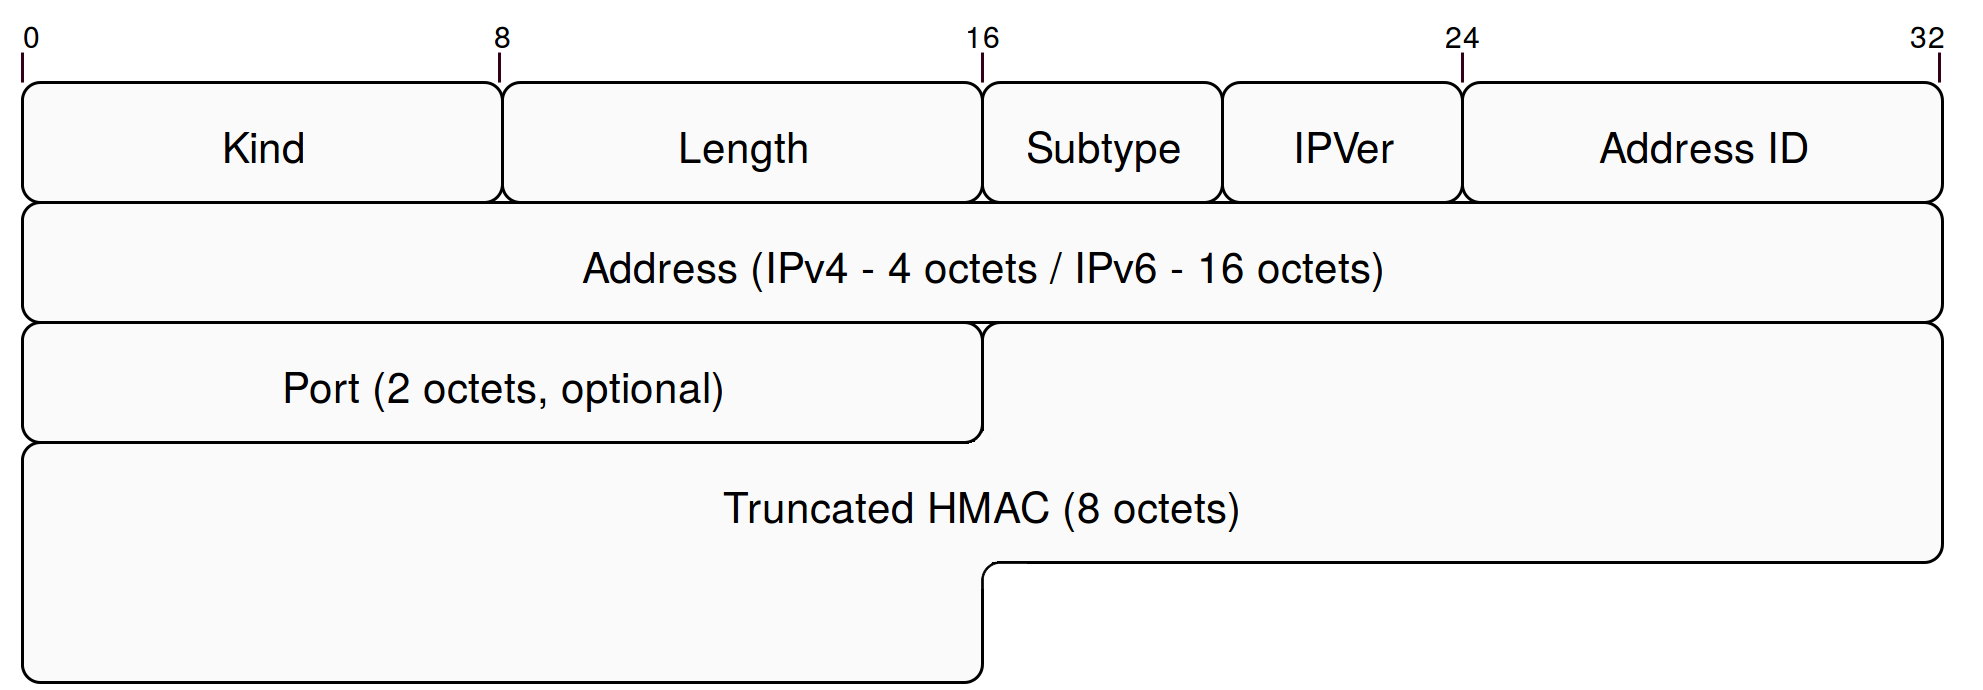
\includegraphics[width=0.75\textwidth]{images/addaddr2}
\caption{ADD\_ADDR2 option}
\label{fig:addaddr2}
\end{figure}

Such format would require the attacker to know the key in order to forge a valid ADD\_ADDR2 message, but such key is not exposed as in the case of the previous solution. Albeit, if the attacker is able to eavesdrop the keys during connection initiation it would be possible to exploit the same vulnerability even with the new address format. More experiments about this case are reported in section [ref to the experimental evaluation section]. Possible mitigations for such threat are explained in section [ref to keys' eavesdrop section 3.3.2].

The keys' eavesdrop threat is a partial-time on-path eavesdrop, a category that is considered less critical in terms of security concerns. Such keys' eavesdrop procedure in MPTCP has an almost identical counterpart in SCTP, when the SCTP-AUTH extension is used without pre-shared keys [\rfc{5061}]. In these regards the same security levels of SCTP would be reached in MPTCP by upgrading ADD\_ADDR to ADD\_ADDR2. Since SCTP is Standard Track, ADD\_ADDR2 is indeed considered a sufficient modification of the MPTCP first design to reach the security levels required for the transition to Standard Track.

\section{Implementing ADD\_ADDR2}
The current MPTCP patch added to the TCP stack in the Linux kernel currently counts around 12000 lines of code [\href{http://multipath-tcp.org/mptcp_stats/index.html}{href}]. The main architectural concepts are now explained, before introducing the modifications related to the new ADD\_ADDR2 format. 


With MPTCP, three main layers are introduced to guarantee multipath management and retro-compatibility with regular TCP [\href{http://inl.info.ucl.ac.be/publications/multipath-tcp-theory-practice}{href}]. The first element is the \textit{master subsocket}, which provides the interface used by the applications to communicate with the TCP stack. The structure of the master subsocket follows the regular TCP standards, in order to maintain retro-compatibility towards the application layer: in fact this is the only element used by the kernel in case of regular TCP connectivity. 

\subsection{Retro-compatibility}
Version control mechanism was not present but it is needed to negotiate which format to use in a MPTCP session: ADD\_ADDR or ADD\_ADDR2.

\subsection{Port advertisement}
Port advertisement in ADD\_ADDR is possible according to RFC specifications but it was not part of the implementation at the beginning of the thesis work, so it has been added.

\subsection{IPv6 considerations}
Longer addresses brought some issues related to TCP option fields limitations.

\subsection{Crypto-API in MPTCP}
A major problem was how to deal with the new hashing requirements introduced by ADD\_ADDR2. Extending the current MPTCP hashing function to deal with input messages of arbitrary size is a first point to explain. The second part has to deal with the whole analysis related to adopting the kernel CRYPTO APIs to calculate the HMAC values in MPTCP and why this is not advisable.

\section{Other contributions}
Another minor part of the thesis work on MPTCP is related to some small contributions to the official RFC documentation and other open-source projects.

\section{Experimental evaluation}
This part should include performance analysis regarding the new format introduced with ADD\_ADDR2. A discussion on how the new format (and all the other modifications introduced with the patches) could impact any aspect of the protocol should be present in this section.
It is possible to add here the other possible solutions for ADD\_ADDR fix, and why they are not good enough. 
\chapter{Conclusions}
\label{chap:conclusions}

\section{Related work}
This thesis is focused on the development of the first implementation of ADD\_ADDR2. No other implementations for such new format have been released yet at the time of writing, even if the specifications for it are currently available in RFC draft documents. This work is closely related to the underlying specifications elaborated by the IETF working group and MPTCP maintainers. From a more general perspective, all the research carried out on the security aspects of MPTCP can be considered related work and this includes middleboxes testing, which is a parallel project active at the Intel office in Lund (Sweden) where this thesis work has been performed. 

\section{Future work}
\label{future}
This thesis workflow mainly involved actual development and testing. The final produced patches have been applied to the official Linux Kernel MPTCP repository, thus marking the first step towards the implementation of the new version of the protocol: MPTCP version 1. 
Both the implementation of MPTCP and the definition of the protocol's specifications are important works in progress for the Internet community. The introduced modifications in this thesis use \rfc{6824bis-04} as reference document, but during the last part of the working period a new RFC draft has been released (\rfc{6824bis-05}) with new MPTCP functionalities and a slightly different implementation of ADD\_ADDR2 as well. A future work will be to update the current ADD\_ADDR2 implementation to follow the new draft document's specifications, keeping in mind that the whole project is at a experimental stage and subjected to relatively frequent modifications.

Another open problem left by this work is the investigation about the Crypto APIs usage in MPTCP, a context that is also found in the SCTP protocol implementation for Linux: since Crypto-API is unsafe in atomic context, current SCTP code must be updated to cope with this aspect. If the problem is definitely solved for SCTP and Crypto-APIs are certified to be safe in SCTP, then it is possible adopt the same code elsewhere in the network components of Linux, including MPTCP. The positive aspect of switching to an already available and established set of cryptographic functions include code re-usability and modularity. Performance comparisons should be investigated as well.

Future work includes the updating of the networking tools in order to be compatible with the new format of ADD\_ADDR. Examples for this have been shown in the thesis for Wireshark and the Nimai's MPTCP-compatible Scapy tool.

Lastly, it is worth mentioning that this paper is focused on the ADD\_ADDR vulnerability, but other threats have been detected for MPTCP. Security concerns will remain one of the main aspects to be investigated and verified during the development phase of MPTCP, so that all the minimum requirements are met before the protocol is added to the public Linux Kernel. This thesis only marginally mention other security implications other than ADD\_ADDR. Moreover, the experimental evaluation reported in this paper addresses the flooding attack considerations related to ADD\_ADDR2, but further studies should be carried out regarding the new format to assess that it does not indeed introduce new attacking vectors or unexpected performance degradation in MPTCP.

\appendix
% INCLUSIONE APPENDICI - - PERSONALIZZARE - TENERE COERENTE CON LISTA IN ALTO
\chapter{ADD\_ADDR attack capture}
\label{app:a}

This appendix contains the capture file for the ADD\_ADDR attack execution as described in chapter \ref{chap:addaddrattackexecution}. This capture is obtained by monitoring \textit{tap0} (targeted interface) and trimmed to just show the TCP flags and the MPTCP options exchanged in signaling packets.

From the capture file it is possible to find the ADD\_ADDR message received from the attacker (frame 21) and the subsequent SYN+MP\_JOIN message sent by the client to the advertised address 10.1.1.1 (frame 22). Moreover, the last frame (frame 30) shows the RST message sent by the attacker to close the subflow, as that is the last step of the hijacking procedure.

\begingroup
    \fontsize{8pt}{9pt}\selectfont
	\begin{verbatim}

...
----------------------------------------------------------------------------------------------------
Frame 2: 86 bytes on wire (688 bits), 86 bytes captured (688 bits)
Ethernet II, Src: 36:92:62:7e:a3:aa (36:92:62:7e:a3:aa), Dst: a6:34:88:29:79:30 (a6:34:88:29:79:30)
Internet Protocol Version 4, Src: 10.1.1.2, Dst: 10.2.1.2
Transmission Control Protocol, Src Port: 59297, Dst Port: 33443, Seq: 0, Len: 0
    ...
    Flags: 0x002 (SYN)
    ...
        Multipath TCP: Multipath Capable
            Kind: Multipath TCP (30)
            Length: 12
            0000 .... = Multipath TCP subtype: Multipath Capable (0)
            .... 0000 = Multipath TCP version: 0
            Multipath TCP flags: 0x81
                1... .... = Checksum required: 1
                .0.. .... = Extensibility: 0
                .... ...1 = Use HMAC-SHA1: 1
                ..00 000. = Reserved: 0x00
            Sender's Key: 16701209312697411725
    ...
----------------------------------------------------------------------------------------------------
Frame 3: 86 bytes on wire (688 bits), 86 bytes captured (688 bits)
Ethernet II, Src: a6:34:88:29:79:30 (a6:34:88:29:79:30), Dst: 36:92:62:7e:a3:aa (36:92:62:7e:a3:aa)
Internet Protocol Version 4, Src: 10.2.1.2, Dst: 10.1.1.2
Transmission Control Protocol, Src Port: 33443, Dst Port: 59297, Seq: 0, Ack: 1, Len: 0
    ...
    Flags: 0x012 (SYN, ACK)
    ...
        Multipath TCP: Multipath Capable
            Kind: Multipath TCP (30)
            Length: 12
            0000 .... = Multipath TCP subtype: Multipath Capable (0)
            .... 0000 = Multipath TCP version: 0
            Multipath TCP flags: 0x81
                1... .... = Checksum required: 1
                .0.. .... = Extensibility: 0
                .... ...1 = Use HMAC-SHA1: 1
                ..00 000. = Reserved: 0x00
            Sender's Key: 1243510374397414024
    ...
----------------------------------------------------------------------------------------------------
Frame 4: 94 bytes on wire (752 bits), 94 bytes captured (752 bits)
Ethernet II, Src: 36:92:62:7e:a3:aa (36:92:62:7e:a3:aa), Dst: a6:34:88:29:79:30 (a6:34:88:29:79:30)
Internet Protocol Version 4, Src: 10.1.1.2, Dst: 10.2.1.2
Transmission Control Protocol, Src Port: 59297, Dst Port: 33443, Seq: 1, Ack: 1, Len: 0
    ...
    Flags: 0x010 (ACK)
    ...
        Multipath TCP: Multipath Capable
            Kind: Multipath TCP (30)
            Length: 20
            0000 .... = Multipath TCP subtype: Multipath Capable (0)
            .... 0000 = Multipath TCP version: 0
            Multipath TCP flags: 0x81
                1... .... = Checksum required: 1
                .0.. .... = Extensibility: 0
                .... ...1 = Use HMAC-SHA1: 1
                ..00 000. = Reserved: 0x00
            Sender's Key: 16701209312697411725
    ...
----------------------------------------------------------------------------------------------------
Frame 5: 87 bytes on wire (696 bits), 87 bytes captured (696 bits)
Ethernet II, Src: 36:92:62:7e:a3:aa (36:92:62:7e:a3:aa), Dst: a6:34:88:29:79:30 (a6:34:88:29:79:30)
Internet Protocol Version 4, Src: 10.1.1.2, Dst: 10.2.1.2
Transmission Control Protocol, Src Port: 59297, Dst Port: 33443, Seq: 1, Ack: 1, Len: 1
    ...
    Flags: 0x018 (PSH, ACK)
    ...
        Multipath TCP: Data Sequence Signal
            Kind: Multipath TCP (30)
            Length: 20
            0010 .... = Multipath TCP subtype: Data Sequence Signal (2)
            Multipath TCP flags: 0x05
                ...0 .... = DATA_FIN: 0
                .... 0... = Data Sequence Number is 8 octets: 0
                .... .1.. = Data Sequence Number, Subflow Sequence Number, Data-level Length, Checksum present: 1
                .... ..0. = Data ACK is 8 octets: 0
                .... ...1 = Data ACK is present: 1
            Original MPTCP Data ACK: 2078391628
            Data Sequence Number: 2995440535  (32bits version)
            Subflow Sequence Number: 1
            Data-level Length: 1
    ...
----------------------------------------------------------------------------------------------------
... [Regular data transfer here]
----------------------------------------------------------------------------------------------------
Frame 21: 62 bytes on wire (496 bits), 62 bytes captured (496 bits)
Ethernet II, Src: a6:34:88:29:79:30 (a6:34:88:29:79:30), Dst: 36:92:62:7e:a3:aa (36:92:62:7e:a3:aa)
Internet Protocol Version 4, Src: 10.2.1.2, Dst: 10.1.1.2
Transmission Control Protocol, Src Port: 33443, Dst Port: 59297, Seq: 1004, Ack: 4294966299, Len: 0
    ...
    Flags: 0x010 (ACK)
    ...
        Multipath TCP: Add Address
            Kind: Multipath TCP (30)
            Length: 8
            0011 .... = Multipath TCP subtype: Add Address (3)
            .... 0100 = IP version: 4
            Address ID: 6
            Advertised IPv4 Address: 10.1.1.1
    ...
----------------------------------------------------------------------------------------------------
Frame 22: 86 bytes on wire (688 bits), 86 bytes captured (688 bits)
Ethernet II, Src: 36:92:62:7e:a3:aa (36:92:62:7e:a3:aa), Dst: a6:34:88:29:79:30 (a6:34:88:29:79:30)
Internet Protocol Version 4, Src: 10.1.1.2, Dst: 10.1.1.1
Transmission Control Protocol, Src Port: 53953, Dst Port: 33443, Seq: 0, Len: 0
    ...
    Flags: 0x002 (SYN)
    ...
        Multipath TCP: Join Connection
            Kind: Multipath TCP (30)
            Length: 12
            0001 .... = Multipath TCP subtype: Join Connection (1)
            Multipath TCP flags: 0x10
                ...1 .... = Backup flag: 1
            Address ID: 2
            Receiver's Token: 1242546132
            Sender's Random Number: 3113663070
    ...
----------------------------------------------------------------------------------------------------
... [TCP retranmission here]
----------------------------------------------------------------------------------------------------
Frame 24: 90 bytes on wire (720 bits), 90 bytes captured (720 bits)
Ethernet II, Src: a6:34:88:29:79:30 (a6:34:88:29:79:30), Dst: 36:92:62:7e:a3:aa (36:92:62:7e:a3:aa)
Internet Protocol Version 4, Src: 10.1.1.1, Dst: 10.1.1.2
Transmission Control Protocol, Src Port: 33443, Dst Port: 53953, Seq: 0, Ack: 1, Len: 0
    ...
    Flags: 0x012 (SYN, ACK)
    ...
        Multipath TCP: Join Connection
            Kind: Multipath TCP (30)
            Length: 16
            0001 .... = Multipath TCP subtype: Join Connection (1)
            Multipath TCP flags: 0x10
                ...1 .... = Backup flag: 1
            Address ID: 4098
            Sender's Truncated HMAC: 2867407674975684266
            Sender's Random Number: 1275303205
    ...
----------------------------------------------------------------------------------------------------
Frame 25: 90 bytes on wire (720 bits), 90 bytes captured (720 bits)
Ethernet II, Src: 36:92:62:7e:a3:aa (36:92:62:7e:a3:aa), Dst: a6:34:88:29:79:30 (a6:34:88:29:79:30)
Internet Protocol Version 4, Src: 10.1.1.2, Dst: 10.1.1.1
Transmission Control Protocol, Src Port: 53953, Dst Port: 33443, Seq: 1, Ack: 1, Len: 0
    ...
    Flags: 0x010 (ACK)
    ...
        Multipath TCP: Join Connection
            Kind: Multipath TCP (30)
            Length: 24
            0001 .... = Multipath TCP subtype: Join Connection (1)
            .... 0000 0000 0000 = Reserved: 0x0000
            Sender's HMAC: 20767a5fd16ca5a23e652f78620883acfbca2590
    ...
----------------------------------------------------------------------------------------------------
...
----------------------------------------------------------------------------------------------------
Frame 30: 54 bytes on wire (432 bits), 54 bytes captured (432 bits)
Ethernet II, Src: a6:34:88:29:79:30 (a6:34:88:29:79:30), Dst: 36:92:62:7e:a3:aa (36:92:62:7e:a3:aa)
Internet Protocol Version 4, Src: 10.2.1.2, Dst: 10.1.1.2
Transmission Control Protocol, Src Port: 33443, Dst Port: 59297, Seq: 4, Len: 0
    ...
    Flags: 0x004 (RST)
    ...
	\end{verbatim}
\endgroup
\chapter{MPTCP version 1 capture}
\label{app:b}

This appendix contains the first 10 packets of a MPTCP connection between two UML virtual machines using the IPv6 network scenario shown in figure \ref{fig:netip6_2}. The MPTCP version in use includes the set of patches developed during the thesis work (compliant with \rfc{6824bis-04}), such as version control (set to 1, as shown in the first three frames related to the MP\_CAPABLE handshake) and ADD\_ADDR2 (the truncated HMAC value is present in frame 4). The main purpose of this capture file is to show the proper functioning of the patches introduced during the thesis work.

The capture file is generated with the Wireshark tool made compatible with ADD\_ADDR2, and the displayed content is trimmed to just show the TCP flags and the MPTCP options exchanged in signaling packets. This capture is obtained by monitoring \textit{tap0}.

\begingroup
    \fontsize{8pt}{9pt}\selectfont
	\begin{verbatim}
Frame 1: 106 bytes on wire (848 bits), 106 bytes captured (848 bits) on interface 0
Ethernet II, Src: c6:c3:59:b0:f2:e6 (c6:c3:59:b0:f2:e6), Dst: 4e:7f:57:76:1a:e4 (4e:7f:57:76:1a:e4)
Internet Protocol Version 6, Src: 1000:1:1::2, Dst: 1000:2:1::2
Transmission Control Protocol, Src Port: 59883, Dst Port: 5001, Seq: 0, Len: 0
    ...
    Flags: 0x002 (SYN)
    ...
        Multipath TCP: Multipath Capable
            Kind: Multipath TCP (30)
            Length: 12
            0000 .... = Multipath TCP subtype: Multipath Capable (0)
            .... 0001 = Multipath TCP version: 1
            Multipath TCP flags: 0x81
                1... .... = Checksum required: 1
                .0.. .... = Extensibility: 0
                .... ...1 = Use HMAC-SHA1: 1
                ..00 000. = Reserved: 0x00
            Sender's Key: 5002747019653015322
    ...
----------------------------------------------------------------------------------------------------
Frame 2: 106 bytes on wire (848 bits), 106 bytes captured (848 bits) on interface 0
Ethernet II, Src: 4e:7f:57:76:1a:e4 (4e:7f:57:76:1a:e4), Dst: c6:c3:59:b0:f2:e6 (c6:c3:59:b0:f2:e6)
Internet Protocol Version 6, Src: 1000:2:1::2, Dst: 1000:1:1::2
Transmission Control Protocol, Src Port: 5001, Dst Port: 59883, Seq: 0, Ack: 1, Len: 0
    ...
    Flags: 0x012 (SYN, ACK)
    ...
        Multipath TCP: Multipath Capable
            Kind: Multipath TCP (30)
            Length: 12
            0000 .... = Multipath TCP subtype: Multipath Capable (0)
            .... 0001 = Multipath TCP version: 1
            Multipath TCP flags: 0x81
                1... .... = Checksum required: 1
                .0.. .... = Extensibility: 0
                .... ...1 = Use HMAC-SHA1: 1
                ..00 000. = Reserved: 0x00
            Sender's Key: 9989746376998273982
    ...
----------------------------------------------------------------------------------------------------
Frame 3: 114 bytes on wire (912 bits), 114 bytes captured (912 bits) on interface 0
Ethernet II, Src: c6:c3:59:b0:f2:e6 (c6:c3:59:b0:f2:e6), Dst: 4e:7f:57:76:1a:e4 (4e:7f:57:76:1a:e4)
Internet Protocol Version 6, Src: 1000:1:1::2, Dst: 1000:2:1::2
Transmission Control Protocol, Src Port: 59883, Dst Port: 5001, Seq: 1, Ack: 1, Len: 0
    ...
    Flags: 0x010 (ACK)
    ...
        Multipath TCP: Multipath Capable
            Kind: Multipath TCP (30)
            Length: 20
            0000 .... = Multipath TCP subtype: Multipath Capable (0)
            .... 0001 = Multipath TCP version: 1
            Multipath TCP flags: 0x81
                1... .... = Checksum required: 1
                .0.. .... = Extensibility: 0
                .... ...1 = Use HMAC-SHA1: 1
                ..00 000. = Reserved: 0x00
            Sender's Key: 5002747019653015322
            Receiver's Key: 9989746376998273982
        Multipath TCP: Data Sequence Signal
            Kind: Multipath TCP (30)
            Length: 8
            0010 .... = Multipath TCP subtype: Data Sequence Signal (2)
            Multipath TCP flags: 0x01
                ...0 .... = DATA_FIN: 0
                .... 0... = Data Sequence Number is 8 octets: 0
                .... .0.. = Data Sequence Number, Subflow Sequence Number, Data-level Length, Checksum present: 0
                .... ..0. = Data ACK is 8 octets: 0
                .... ...1 = Data ACK is present: 1
            Original MPTCP Data ACK: 872094606
    ...
----------------------------------------------------------------------------------------------------
Frame 4: 114 bytes on wire (912 bits), 114 bytes captured (912 bits) on interface 0
Ethernet II, Src: 4e:7f:57:76:1a:e4 (4e:7f:57:76:1a:e4), Dst: c6:c3:59:b0:f2:e6 (c6:c3:59:b0:f2:e6)
Internet Protocol Version 6, Src: 1000:2:1::2, Dst: 1000:1:1::2
Transmission Control Protocol, Src Port: 5001, Dst Port: 59883, Seq: 1, Ack: 1, Len: 0
    ...
    Flags: 0x010 (ACK)
    ...
        Multipath TCP: Add Address
            Kind: Multipath TCP (30)
            Length: 28
            0011 .... = Multipath TCP subtype: Add Address (3)
            .... 0110 = IP version: 6
            Address ID: 8
            Advertised IPv6 Address: 1000:2:2::2
            Truncated HMAC: 7594364714824743626
    ...
----------------------------------------------------------------------------------------------------
Frame 5: 130 bytes on wire (1040 bits), 130 bytes captured (1040 bits) on interface 0
Ethernet II, Src: c6:c3:59:b0:f2:e6 (c6:c3:59:b0:f2:e6), Dst: 4e:7f:57:76:1a:e4 (4e:7f:57:76:1a:e4)
Internet Protocol Version 6, Src: 1000:1:1::2, Dst: 1000:2:1::2
Transmission Control Protocol, Src Port: 59883, Dst Port: 5001, Seq: 1, Ack: 1, Len: 24
    ...
    Flags: 0x018 (PSH, ACK)
    ...
        Multipath TCP: Data Sequence Signal
            Kind: Multipath TCP (30)
            Length: 20
            0010 .... = Multipath TCP subtype: Data Sequence Signal (2)
            Multipath TCP flags: 0x05
                ...0 .... = DATA_FIN: 0
                .... 0... = Data Sequence Number is 8 octets: 0
                .... .1.. = Data Sequence Number, Subflow Sequence Number, Data-level Length, Checksum present: 1
                .... ..0. = Data ACK is 8 octets: 0
                .... ...1 = Data ACK is present: 1
            Original MPTCP Data ACK: 872094606
            Data Sequence Number: 3712008769  (32bits version)
            Subflow Sequence Number: 1
            Data-level Length: 24
    ...
----------------------------------------------------------------------------------------------------
Frame 6: 94 bytes on wire (752 bits), 94 bytes captured (752 bits) on interface 0
Ethernet II, Src: 4e:7f:57:76:1a:e4 (4e:7f:57:76:1a:e4), Dst: c6:c3:59:b0:f2:e6 (c6:c3:59:b0:f2:e6)
Internet Protocol Version 6, Src: 1000:2:1::2, Dst: 1000:1:1::2
Transmission Control Protocol, Src Port: 5001, Dst Port: 59883, Seq: 1, Ack: 25, Len: 0
    ...
    Flags: 0x010 (ACK)
    ...
        Multipath TCP: Data Sequence Signal
            Kind: Multipath TCP (30)
            Length: 8
            0010 .... = Multipath TCP subtype: Data Sequence Signal (2)
            Multipath TCP flags: 0x01
                ...0 .... = DATA_FIN: 0
                .... 0... = Data Sequence Number is 8 octets: 0
                .... .0.. = Data Sequence Number, Subflow Sequence Number, Data-level Length, Checksum present: 0
                .... ..0. = Data ACK is 8 octets: 0
                .... ...1 = Data ACK is present: 1
            Original MPTCP Data ACK: 3712008793
    ...
----------------------------------------------------------------------------------------------------
Frame 7: 106 bytes on wire (848 bits), 106 bytes captured (848 bits) on interface 0
Ethernet II, Src: c6:c3:59:b0:f2:e6 (c6:c3:59:b0:f2:e6), Dst: 4e:7f:57:76:1a:e4 (4e:7f:57:76:1a:e4)
Internet Protocol Version 6, Src: 1000:1:1::2, Dst: 1000:2:2::2
Transmission Control Protocol, Src Port: 45840, Dst Port: 5001, Seq: 0, Len: 0
    ...
    Flags: 0x002 (SYN)
    ...
        Multipath TCP: Join Connection
            Kind: Multipath TCP (30)
            Length: 12
            0001 .... = Multipath TCP subtype: Join Connection (1)
            Multipath TCP flags: 0x10
                ...1 .... = Backup flag: 1
            Address ID: 8
            Receiver's Token: 4008023058
            Sender's Random Number: 4053633689
    ...
----------------------------------------------------------------------------------------------------
Frame 8: 110 bytes on wire (880 bits), 110 bytes captured (880 bits) on interface 0
Ethernet II, Src: 4e:7f:57:76:1a:e4 (4e:7f:57:76:1a:e4), Dst: c6:c3:59:b0:f2:e6 (c6:c3:59:b0:f2:e6)
Internet Protocol Version 6, Src: 1000:2:2::2, Dst: 1000:1:1::2
Transmission Control Protocol, Src Port: 5001, Dst Port: 45840, Seq: 0, Ack: 1, Len: 0
    ...
    Flags: 0x012 (SYN, ACK)
    ...
        Multipath TCP: Join Connection
            Kind: Multipath TCP (30)
            Length: 16
            0001 .... = Multipath TCP subtype: Join Connection (1)
            Multipath TCP flags: 0x10
                ...1 .... = Backup flag: 1
            Address ID: 4104
            Sender's Truncated HMAC: 16644964641649406387
            Sender's Random Number: 3923749318
    ...
----------------------------------------------------------------------------------------------------
Frame 9: 110 bytes on wire (880 bits), 110 bytes captured (880 bits) on interface 0
Ethernet II, Src: c6:c3:59:b0:f2:e6 (c6:c3:59:b0:f2:e6), Dst: 4e:7f:57:76:1a:e4 (4e:7f:57:76:1a:e4)
Internet Protocol Version 6, Src: 1000:1:1::2, Dst: 1000:2:2::2
Transmission Control Protocol, Src Port: 45840, Dst Port: 5001, Seq: 1, Ack: 1, Len: 0
    ...
    Flags: 0x010 (ACK)
    ...
        Multipath TCP: Join Connection
            Kind: Multipath TCP (30)
            Length: 24
            0001 .... = Multipath TCP subtype: Join Connection (1)
            .... 0000 0000 0000 = Reserved: 0x0000
            Sender's HMAC: 95d50d4aa4861fb5adccd0b92017622fa0275f29
    ...
----------------------------------------------------------------------------------------------------
Frame 10: 94 bytes on wire (752 bits), 94 bytes captured (752 bits) on interface 0
Ethernet II, Src: 4e:7f:57:76:1a:e4 (4e:7f:57:76:1a:e4), Dst: c6:c3:59:b0:f2:e6 (c6:c3:59:b0:f2:e6)
Internet Protocol Version 6, Src: 1000:2:2::2, Dst: 1000:1:1::2
Transmission Control Protocol, Src Port: 5001, Dst Port: 45840, Seq: 1, Ack: 1, Len: 0
    ...
    Flags: 0x010 (ACK)
    ...
        Multipath TCP: Data Sequence Signal
            Kind: Multipath TCP (30)
            Length: 8
            0010 .... = Multipath TCP subtype: Data Sequence Signal (2)
            Multipath TCP flags: 0x01
                ...0 .... = DATA_FIN: 0
                .... 0... = Data Sequence Number is 8 octets: 0
                .... .0.. = Data Sequence Number, Subflow Sequence Number, Data-level Length, Checksum present: 0
                .... ..0. = Data ACK is 8 octets: 0
                .... ...1 = Data ACK is present: 1
            Original MPTCP Data ACK: 3712008793
    ...

	\end{verbatim}
\endgroup

%%%%%%%%%%%%%%%%%%%%%%%%%%%%%%%%%%%%%%%%%%%%%%%%%%%%%%%%%%%%%%%

% BIBLIOGRAFIA
\addcontentsline{toc}{chapter}{\refname}
\nocite{*}
\printbibliography

\end{document}